\RequirePackage[switch, columnwise, running, mathlines, displaymath,
mathlines]{lineno}
\RequirePackage{docswitch}
% \flag is set by the user, through the makefile:
%    make note
%    make apj
% etc.
\setjournal{\flag}

\documentclass[\docopts]{\docclass}

\newcommand*\patchAmsMathEnvironmentForLineno[1]{%
  \expandafter\let\csname old#1\expandafter\endcsname\csname #1\endcsname
  \expandafter\let\csname oldend#1\expandafter\endcsname\csname end#1\endcsname
  \renewenvironment{#1}%
     {\linenomath\csname old#1\endcsname}%
     {\csname oldend#1\endcsname\endlinenomath}}%
\newcommand*\patchBothAmsMathEnvironmentsForLineno[1]{%
  \patchAmsMathEnvironmentForLineno{#1}%
  \patchAmsMathEnvironmentForLineno{#1*}}%
\AtBeginDocument{%
\patchBothAmsMathEnvironmentsForLineno{equation}%
\patchBothAmsMathEnvironmentsForLineno{align}%
\patchBothAmsMathEnvironmentsForLineno{flalign}%
\patchBothAmsMathEnvironmentsForLineno{alignat}%
\patchBothAmsMathEnvironmentsForLineno{gather}%
\patchBothAmsMathEnvironmentsForLineno{multline}%
}

% You could also define the document class directly
%\documentclass[]{emulateapj}

% Custom commands from LSST DESC, see texmf/styles/lsstdesc_macros.sty
\usepackage{lsstdesc_macros}
% \usepackage{natbib}
% \usepackage{subcaption}
\usepackage[colorinlistoftodos]{todonotes}
% \usepackage[colorlinks=true, allcolors=blue]{hyperref}
\usepackage{multirow}
\usepackage{xspace}
\usepackage{enumitem}
\usepackage{graphicx}
\usepackage{wasysym}
\usepackage{amsmath}
\usepackage{amssymb}
\usepackage{amsfonts}
\usepackage{footmisc}
\graphicspath{{./}{./figures/}}
\bibliographystyle{mnras}%mn2e

% Add your own macros here:
\newcommand{\textul}{\underline}

% projects
\newcommand{\proj}[1]{\textsc{#1}}
\newcommand{\lsst}{\proj{LSST}}
\newcommand{\lsstdesc}{\lsst-\proj{DESC}}
\newcommand{\sdss}{\proj{SDSS}}
\newcommand{\buzz}{\proj{Buzzard}}

% can easily change these to specify posterior throughout, etc
\newcommand{\pz}{photo-$z$}
\newcommand{\pzpdf}{\pz\ PDF}
\newcommand{\Pz}{Photo-$z$}
\newcommand{\Pzpdf}{\Pz\ PDF}
\newcommand{\chisq}{$\chi^{2}$}

% codes
\newcommand{\pzcode}[1]{\texttt{#1}}
\newcommand{\qp}{\pzcode{qp}}
\newcommand{\annz}{\pzcode{ANNz2}}
\newcommand{\bpz}{\pzcode{BPZ}}
\newcommand{\cmnn}{\pzcode{CMNN}}
\newcommand{\delight}{\pzcode{Delight}}
\newcommand{\eazy}{\pzcode{EAZY}}
\newcommand{\flexzboost}{\pzcode{FlexZBoost}}
\newcommand{\gpz}{\pzcode{GPz}}
\newcommand{\lephare}{\pzcode{LePhare}}
\newcommand{\metaphor}{\pzcode{METAPhoR}}
\newcommand{\skynet}{\pzcode{SkyNet}}
\newcommand{\tpz}{\pzcode{TPZ}}
\newcommand{\trainz}{\pzcode{trainZ}}

\newcommand*\mathinhead[2]{\texorpdfstring{$\boldsymbol{#1}$}{#2}}

\newcommand{\red}[1]{\textcolor{red}{#1}}
% Claim a color for your comments
\newcommand{\aim}[1]{\textcolor{green}{#1}}%Alex Malz comments in green
\newcommand{\blue}[1]{\textcolor{blue}{#1}}%unknown person comments in blue
\definecolor{scc}{rgb}{0.0, 0.26, 0.15}
\newcommand{\scc}[1]{\textcolor{scc}{#1}}%Stefano Cavuoti Comments in dark green
\definecolor{newpink}{rgb}{0.858, 0.188, 0.478}
\newcommand{\erfan}[1]{\textcolor{newpink}{#1}} % Erfan Nourbakhsh comments in pink
\newcommand{\jan}[1]{\textcolor{orange}{#1}}%Jeff Newman comments in Orange

\def\X{{\mathbf{X}}}
\def\x{{\mathbf{x}}}
\def\E{{\mathbb{E}}}

% ======================================================================
%\hypersetup{draft}
\begin{document}
\linenumbers

\title{Evaluation of probabilistic photometric redshift estimation approaches for \textsc{LSST}}

\maketitlepre

\begin{abstract}

Many scientific investigations of photometric galaxy surveys require redshift estimates, whose uncertainty properties are best encapsulated by photometric redshift (photo-$z$) posterior probability distribution functions (PDFs).
A plethora of photo-$z$ PDF estimation methodologies abound, producing discrepant results with no consensus on a preferred approach.
We present the results of a comprehensive experiment comparing twelve photo-$z$ algorithms applied to mock data produced for the Large Synoptic Survey Telescope (\textsc{LSST}) Dark Energy Science Collaboration (\textsc{DESC}).
By supplying perfect prior information, in the form of the complete template library and a representative training set as inputs to each code, we demonstrate the impact of the assumptions underlying each technique on the output photo-$z$ PDFs.
In the absence of a notion of true, unbiased photo-$z$ PDFs, we evaluate and interpret multiple metrics of the ensemble properties of the derived photo-$z$ PDFs as well as traditional reductions to photo-$z$ point estimates.
We report systematic biases and overall over/under-breadth of the photo-$z$ PDFs of many popular codes, which may indicate avenues for improvement in the algorithms or implementations.
Furthermore, we raise attention to the limitations of established metrics for assessing photo-$z$ PDF accuracy; though we identify the conditional density estimate (CDE) loss as a promising metric of photo-$z$ PDF performance in the case where true redshifts are available but true photo-$z$ PDFs are not, we emphasize the need for science-specific performance metrics.

\end{abstract}

% Keywords are ignored in the LSST DESC Note style:
\dockeys{galaxies: distances and redshifts -- galaxies: statistics -- methods: statistical}

\maketitlepost

% ----------------------------------------------------------------------
% 

\section{Introduction}
\label{sec:intro}

The current and next generations of large-scale galaxy surveys, including the Dark Energy Survey \citep[\textsc{DES},][]{Abbott:05}, the Kilo-Degree Survey \citep[\textsc{KiDS},][]{de_Jong:13}, Hyper Suprime-Cam Survey \citep[\textsc{HSC},][]{Aihara:2018a,Aihara:2018b}, Large Synoptic Survey Telescope \citep[\lsst,][]{Abell:09}, Euclid \citep{Laureijs:11}, and Wide-Field Infrared Survey Telescope \citep[\textsc{WFIRST},][]{Green:12}, present a paradigm shift from spectroscopic to photometric galaxy catalogs of substantially larger size at a cost of lacking complete spectroscopically confirmed redshifts.

Effective astrophysical inference using the catalogs resulting from these ongoing and upcoming missions, however, necessitates accurate and precise photometric redshift (\pz) estimation methodologies.
As an example, in order for \pz\ systematics to not dominate the statistical noise floor of \lsst's main cosmological sample of $\sim 10^{7}$ galaxies, the \lsst\ Science Requirements Document (SRD)\footnote{available at \url{https://docushare.lsstcorp.org/docushare/dsweb/Get/LPM-17}} specifies that individual galaxy \pz s must have root-mean-square error $\sigma_z < 0.02 (1+z)$, $3 \sigma$ ``catastrophic outlier'' rate below $10\%$, and bias below $0.003$.
Specific science cases may have their own requirements on \pz\ performance that exceed those of the survey as a whole.
In that vein, the \lsst\ Dark Energy Science Collaboration (\lsstdesc) developed a separate SRD \citep{Mandelbaum:2018} that conservatively forecasts the constraining power of five cosmological probes, leading to even more stringent requirements on \pz\ performance, including those defined in terms of tomographically binned subsamples populations rather than individual galaxies.

Though the standard has long been for each galaxy in a photometric catalog to have a \pz\ point estimate and Gaussian error bar, the nontrivial mapping between broad band fluxes and redshift renders this simplistic summary inadequate to quantify the uncertainty landscape by neglecting degenerate redshift solutions.
Far from a hypothetical situation, this degeneracy is a real consequence of the same deep imaging that enables larger galaxy catalog sizes.
The lower luminosity and higher redshift populations captured by deeper imaging introduce major physical systematics to \pz s, among them the Lyman break/Balmer break degeneracy, that did not affect shallower large area surveys like the Sloan Digital Sky Survey \citep[\textsc{SDSS},][]{York:00} and Two Micron All Sky Survey \citep[\textsc{2MASS},][]{Skrutskie:06}.

To fully characterize such physical degeneracies, photometric galaxy catalog data releases from \citep{Mandelbaum:2008} to \citep{de_Jong:17}, provided a more informative \pz\ data product, the \pz\ probability density function (PDF), that describes the relative probability as a function of a galaxy's redshift, conditioned on the observed photometry.
Early template-based methods such as \citet{Fernandezsoto:99} approximated the likelihood of photometry conditioned on redshift with the relative $\chi^{2}$ values of template spectra.
Not long after, Bayesian adaptations of template-based approaches such as \citet{Benitez:00} combined the estimated likelihoods with a prior to yield a posterior PDF of redshift conditioned on photometry.
While the first machine learning based algorithms focused on a point-estimate, \citet{Firth:03} estimated a \pzpdf\ using a neural net with 1000 realizations scattered within the photometric errors.

% MOVE TO WHERE \nz\ IS INTRODUCED AS A METRIC
% For cosmological measurements, certain science cases require redshift information on individual objects, e.~g.~identification of host galaxy redshift for supernova classification, or identifying potential cluster membership.
% Other science cases seem to need only ensemble redshift information; for instance many current cosmic shear techniques require only the overall redshift distribution $N(z)$ for tomographic redshift samples.
% However,  even such cases require individual object redshift estimates for portions of the analysis, for example in determining galaxy intrinsic alignments in weak lensing samples.
% In addition, recent data-driven techniques employing hierarchical Bayesian or Gaussian Process methods have emerged that calibrate redshift distributions using individual $p(z)$ estimates \citep[e.~g.~][]{Sanchez:2018}.
% Techniques for using \pzpdf s have lagged behind the development of codes to produce them, however, all existing approaches assume that the \pzpdf\ for each galaxy is an accurate PDF, with failures when the assumption is violated.
% Thus, even methods that seem to need only ensemble $N(z)$ may actually require accurate $p(z)$ in order to meet stringent survey requirements.
% Large photometric surveys such as LSST must develop algorithms that simultaneously meet the needs of all science cases.
% In order to meet these ambitious goals for photo-$z$ accuracy, every aspect of photo-$z$ estimation will have to be optimized: the algorithms employed, both template and machine-learning based (both in design and implementation); the spectroscopic data used as a training set for machine learning algorithms or to estimate template sets and train Bayesian priors; and probabilistic catalogue compression schemes that balance information retention against limited storage resources.

There are numerous techniques for deriving \pzpdf s, yet no one method has yet been established as clearly superior.
Quantitative comparisons of photo-$z$ methods have been made before.
The Photo-$z$ Accuracy And Testing \citep[\textsc{PHAT},][]{Hildebrandt:10} effort focused on \pz\ point estimates derived from many photometric bands.
\citet{Rau:2015} introduced a new method for improving \pzpdf s using an ordinal classification algorithm.
\textsc{DES} compared several codes for \pz\ point estimates and a subset with \pzpdf\ information \citep{Sanchez:14} and examined summary statistics of \pzpdf s for tomographically binned galaxy subsamples \citep{Bonnett:16}.

This paper is distinguished by its focus on the evaluation criteria for \pzpdf s and interpretation thereof, as part of the mission of the , as a key project of the Photometric Redshift working group of the \lsstdesc\ laid out in the Science Roadmap (SRM)\footnote{Available at: \url{http://lsst-desc.org/sites/default/files/DESC_SRM_V1_1.pdf}}.
In this initial study, we focus on evaluating the performance of \pzpdf\ codes and PDF-specific performance metrics in a controlled experiment with complete and representative prior information (template libraries and training sets).
% Specific implementation choices in each code will influence the resultant posterior distributions, for example choice of prior parameterization in template-based codes, the bandwidth size chosen for machine learning based codes, or even the output format chosen for storing the PDF.
% We have attempted to minimize the impact of many of these factors when comparing codes, for example by using the same template set for all template-based codes, and using a training set that is drawn from the same underlying population as the test sample, to create a controlled environment in which to compare the photo-$z$ PDFs derived from each method.
% We explore a number of performance metrics in this paper that test whether the posterior estimates are actual PDFs.
% Comparing the relative performance of the codes enables us to evaluate whether each code is using information in an optimal way, and may reveal enhancements in some codes and deficiencies in others, either in the fundamental algorithm, or in specific implementation.
% Identifying and fixing failure modes within codes may aid us in reaching the stringent photo-$z$ performance goals set out for LSST.
% We note that these initial tests are a necessary requirement for photo-$z$ codes that will be used in cosmological analyses; however, meeting these requirements is only the first stage in the process, and can be thought of as an initial test under near perfect conditions to test for problems before further complexities are added in future analyses.

The outline of the paper is as follows: in \S\,\ref{sec:sims} we present the simulated data set; in \S\,\ref{sec:pzcodes} we describe the current generation codes employed in the paper; in \S\,\ref{sec:metrics} we discuss the interpretation of photo-$z$ PDFs in terms of metrics of accuracy; in \S\,\ref{sec:results} we show our results and compare the performance of the codes; in \S\,\ref{sec:discussion} we offer our conclusions and discuss future extensions of this work.


\section{The simulation and mock galaxy catalog}
\label{sec:sims}
%(Sam Schmidt, Eve Kovacs, Tina Peters)

In order to test the current generation codes, we employ an existing simulated galaxy catalogue. The simulation is completely catalogue-based, with no image construction or mock measurements made. We describe these in detail below.

\subsection{Buzzard-v1.0 simulation}
\label{sec:buzzard}
The \textsc{Buzzard-highres-v1.0} (De Rose et al., in prep; Wechsler et al., in prep) catalogue construction started with a dark matter only simulation. This N-body simulation contained $2048^3$ particles in a $400$ Mpc h$^{-1}$ box. A set of time snapshots (with smoothing and interpolation between snapshots) were saved in order to construct a lightcone. Dark matter halos were identified using the \textsc{Rockstar} software package \citep{Behroozi:13}. These dark matter halos were populated with galaxies with a stellar mass and absolute $r$-band magnitude in the SDSS system determined using a sub-halo abundance matching model constrained to match both projected two-point galaxy clustering statistics and an observed conditional stellar mass function \citep{Reddick:13}.

To assign an SED to each galaxy, the {\it Adding Density Dependent Spectral Energy Distributions} (\textsc{ADDSEDS}, deRose in prep.)\footnote{\url{https://github.com/vipasu/addseds}} procedure was used. This consisted of training an empirical relation between absolute $r$-band magnitude, local galaxy density, and SED using a sample of $\sim 5\times 10^{5}$ galaxies from the magnitude-limited Sloan Digital Sky Survey Data Release 6 Value Added Galaxy Catalog \citep{Blanton:05}.  Each SDSS spectrum is fit with a sum of five SED components using the \textsc{k-correct \red{v4\_3?}} software package\footnote{\url{http://kcorrect.org}} \citep{Blanton:07}, thus each galaxy SED is parameterized as five weights for the basis SEDs. The distance to the spatial projected fifth-nearest neighbour was used as a proxy for local density in the SDSS training sample. For each simulated galaxy, a galaxy with similar absolute $r$-band magnitude and local galaxy density was chosen from the training set, and that training galaxy's SED was assigned to the simulated galaxy.  This process is done in such a way as to preserve the colour-density relation of galaxy environment.  Given the SED, absolute $r$-band magnitude and redshift, we computed apparent magnitudes in the six LSST filter passbands, $ugrizy$. We assigned magnitude errors in the six bands using the simple model described in \citet{Ivezic:08}, assuming full 10-year depth observations had been completed.  The number of total 30-second visits assumed when generating the photometric errors differs slightly from the fiducial numbers assumed for LSST: we assume 60 visits in u-band, 80 visits in g-band, 180 visits in r-band, 180 visits in i-band, 160 visits in z-band, and 160 visits in y-band.
%numbers taken from Alex Abate's photErrorModel.py script in PhotoZDC1 repository, which was used with nYrObs=10.
In the course of simulating Gaussian photometric errors, we add noise to objects fluxes, and some of these noisy fluxes will become negative in one or more bands.  We call such negative fluxes ``non-detections'' and signify them with a placholder magnitude of 99.0 in the catalog.  Thus, further mentions of ``non-detections'' refer to objects that would be ``looked at but not seen'' in multi-band forced photometry, and the photo-z codes will treat them as such.

\subsubsection{Selection of training and test sets}
\label{sec:buzztraining}
The total catalogue covered $400$ square degrees and contained $238$ million galaxies to an apparent magnitude limit of $r\!=\!29$ and spanning the redshift range $0\!<\!z\!\leq\!8.7$.  In order for statistical errors not to dominate, we need less than one million galaxies in our sample.  Several studies claim that only a few tens of thousands of spectra are necessary to calibrate photo-z surveys to Stage IV requirements (e.~g.~\citet{Bernstein:10}, \citet{Masters:2017}).  Therefore, we aim for a final number of training galaxies between $3\times 10^{4}$ and $5\times 10^{4}$ in our sample.
%This catalogue contained two orders of magnitude more galaxies than were necessary to determine statistics for this study,
In order to reduce our sample to a reasonable size, we limit our dataset to a subset of $\sim\!16.8$ square degrees selected from five separate spatial regions of the simulation. Systematic problems with galaxy colors above $z\!>\!2$ were observed, so the catalogue was limited to include only galaxies in the redshift range $0\!<\!z\!\leq\!2.0$. A random subset of the the remaining galaxies was chosen, and placed at random into either a ``training'' set ($10$ per cent of the sample), for which the galaxies true redshifts will be supplied, or a ``test'' set (the remaining $90$ per cent of the sample), for which each code will need to predict a redshift PDF for each galaxy. %The resulting catalogues contain $111\,171$ training galaxies and $1\,000\,883$ test galaxies.
Finally, we restrict our analysis to a sample with an apparent magnitude limite $i<25.3$, which give a signal-to-noise $\sim\,30$ for most galaxies, a cut often referred to as the expected ``LSST Gold Sample''.  This magnitude cut results in a training set with $44\,404$ galaxies and a test set containing $399\,356$ galaxies.  All subsequent results will evaluate this ``gold sample'' test set.

\subsubsection{Templates}
\label{sec:buzztemplates}
As mentioned in Section~\ref{sec:buzzard}, the SEDs in the Buzzard simulation are drawn from an empirical set of SEDs taken from the SDSS DR6 NYU-VAGC, a sample of roughly $\sim5\times 10^{5}$ galaxies with spectra in SDSS. To determine a finite set of templates to use with template fitting codes we take the five SED weight coefficients for each of the galaxies in the SDSS sample and run a simple K-means clustering algorithm on this five dimensional space. Each dimension was normalized such that it spanned an interval $[0,1]$.  The K-means clusters partition the five-dimensional space of coefficients into Voronoi cells, spanning the space of coefficients in a way that properly reflects the underlying density in the coefficients. Thus, the resultant SEDs constructed using the cell centers as weight coefficients will provide a reasonable spanning SED set. An ad-hoc number of $K=100$ was chosen and the $100$ K-means centre positions are taken as the weights for the \textsc{k-correct} SED components to construct one hundred template SEDs. These $100$ templates were provided,
%\red{(JS: if I remembered correctly, weren't there 150 templates given? Answer: no, initially I supplied a list of 150 that were drawn with a different algorithm, but once we switched to the final k-means set I only supplied 100 (the initial algorithm over-weighted outlier SEDs, which is why we needed the extra 50)--SJS)}
and the templates were used by both \textsc{BPZ} and \textsc{LePhare}; however, because EAZY was designed and written to use the same five basis templates employed by \textsc{k-correct} when constructing our mock galaxies, EAZY was run using linear combinations of these five templates rather than using the 100 discrete templates.  The ability to fit for linear combinations of templates highlights an important implementation difference between similar photo-z codes.


\subsubsection{Limitations}
\label{sec:buzzlimitations}
For our initial investigation of photometric redshift codes, we begin with a data set that is somewhat idealized, and does not contain all of the complicating factors present in real data.  In several cases, the simplification is done with a purpose, with potentially confounding effects excluded in order to better isolate the differences between current-generation photo-$z$ codes, and their causes.  We list several of the simulations limitations in this section.
As the simulation is catalogue-based, no image level effects, such as photometric measurement effects, object blending, contamination from sky background (Zodiacal light, scattered light, etc...), lensing magnification, or Galactic reddening are included.  No stars are included in the catalogue, nor are the effects of AGN.
As all SEDs are constructed from only five basis templates, properties of the galaxy population will be restricted to follow linear combinations of the characteristics of the five basis templates, so certain non-linear features, for example the full range of emission line fluxes relative to the continuum, will not be included in the model galaxy population.  Moreover, the linear combinations of templates are modeled on the $\sim5\times 10^{5}$ SDSS galaxies discussed in Section~\ref{sec:buzzard}, and thus only galaxies that resemble those spectroscopically observed by the SDSS will be included in the sample.  No additional dust reddening intrinsic to the host galaxy is included, the only approximation of dust extinction comes in the form of dust encoded in the five basis SEDs via the training set used to create the basis templates.  Simple linear combinations of these basis templates will, once again, not explore the full range of realistic dust extinction observed in galaxy populations.
While these idealized conditions limit the realism of our galaxy population, some are also by design.  We aim to test the photo-z codes at a very basic level, and a simplified model assures that differences in results seen between the codes are due to fundamental differences in their underlying assumptions and implementation details, rather than more nuanced implementation details.  

%\subsection{ABC-Galacticus simulation}
%\label{sec:galacticus}
%\red{The Argonne-Berkeley-Carnegie (ABC) Galacticus cosmological simulation uses a semi-analytic model to simulate the galaxy properties and is not directly tuned to observations. Each simulated SED is replaced with a SED drawn from the distribution of empirical SEDs given by the SED Atlas of \citet{Brown:14} (diffusion maps method in development).}


\section{Methods}
\label{sec:pzcodes}

Here we summarize the twelve \pzpdf\ codes compared in this study, summarized in Table~\ref{tab:list_of_codes}, which include both established and emerging approaches in template fitting and machine learning.
Though not exhaustive, this sample represents codes for which there was sufficient expertise within the \lsstdesc\ Photometric Redshifts Working Group.  Some aspects of data treatment were left to the individual code runners, for example, whether/how to split the available data with known redshifts into separate training and validation sets. Another key difference is the treatment of non-detections in one or more bands: some codes choose to ignore a band, others replace the value with either an estimate for the detection limit, the mean of other values in the training set, or another default value. There are varying conventions among machine learning based codes for treatment of non-detections, and no one prescription dominates in the photo-z literature. The specific choices for each code affect the results, and contribute to the implicit prior influencing their output. However, we remind the reader that only 2.0 per cent of our sample has non-detections, almost exclusively in the u-band, and thus should not dominate the code performance differences.  The authors welcome interest from those outside \lsstdesc\ to have their codes assessed in future investigations that build upon this one.

\begin{table*}  %%% DATA TABLE %%%
\caption{List of \pzpdf\ codes featured in this study} \label{tab:list_of_codes}\resizebox{\textwidth}{!}{
\begin{tabular}{lll}
\hline
\bf Published code & \bf Type & \bf Public source code \\
\hline
\lephare~\citep{Arnouts:99}	   & template fitting	& \url{http://www.cfht.hawaii.edu/~arnouts/lephare.html} \\
\bpz~\citep{Benitez:00} 		   & template fitting	& \url{http://www.stsci.edu/~dcoe/BPZ/} \\
\eazy~\citep{Brammer:08}		   & template fitting & \url{https://github.com/gbrammer/eazy-photoz} \\
\annz~\citep{Sadeh:16}		     & machine learning	& \url{https://github.com/IftachSadeh/ANNZ} \\
\flexzboost~\citep{Izbicki:17} & machine learning & \url{https://github.com/tpospisi/flexcode}; \url{https://github.com/rizbicki/FlexCoDE}\\
%\textsc{Frankenz} 	& ML 	& \citet{Speagle:frankenz}	& \url{https://github.com/joshspeagle/frankenz} \\
\gpz~\citep{Almosallam:15b}	   & machine learning	& \url{https://github.com/OxfordML/GPz} \\
\metaphor~\citep{Cavuoti:17}   & machine learning	& \url{http://dame.dsf.unina.it}\\
\cmnn~\citep{Graham:17}        & machine learning & N/A \\
\skynet~\citep{Graff:14}       & machine learning & \url{http://ccpforge.cse.rl.ac.uk/gf/project/skynet/} \\
\tpz~\citep{Carrasco_Kind:13}	 & machine learning	& \url{https://github.com/mgckind/MLZ} \\
\delight~\citep{Leistedt:17}   & hybrid           & \url{https://github.com/ixkael/Delight} \\
\hline
\trainz 	                             & machine learning	& See Section~\ref{sec:trainz} \\
\end{tabular}}
\end{table*}

We describe the algorithms and implementations of the model-based and data-driven codes in Sections~\ref{sec:templatecodes} and \ref{sec:trainingcodes} respectively, with a straw-person approach included in Section~\ref{sec:trainz}.
% For each approach, we note how it accounts for photometric uncertainties, how it interprets negative fluxes, what its native output format of \pzpdf s is, and what, if any, preprocessing, including validation, of the prior information it performs.
% In the following sections, we use a consistent notation defined in Table~\ref{tab:variables}.
%
% \begin{table}
% 	\label{tab:variables}
% 	\caption{Definitions of variables used in outlining \pzpdf\ codes}
% 	\begin{tabular}{ll}
% 		\hline
% 		\bf Symbol & \bf Definition \\
% 		\hline
% 		\multirow{ 2}{*}{$b = 1,\dots,B$	& \multirow{ 2}{*}{number $B$ of photometric filters $b$;} \\
% 														& \lsst's $ugrizy$ filters used here correspond to $B=6$ \\
% 		\multirow{ 2}{*}{$m_{b} = 1,\dots,B$	& \multirow{ 2}{*}{number $B$ of photometric filters $b$;} \\
% 																										& \lsst's $ugrizy$ filters used here correspond to $B=6$ \\
% 		$z$											& redshift \\
% 		$T$											& galaxy SED \\
%
% 	\end{tabular}
% \end{table}

\subsection{Template-based Approaches}
\label{sec:templatecodes}

We test three publicly available and commonly used template-based codes that share the standard physically motivated approach of calculating model fluxes for a set of template SEDs on a grid of redshift values and evaluating a \chisq\ merit function using the observed and model fluxes:
\begin{equation} \label{eq_temp_chi}
\chi^2(z,T,A) = \sum_i^{N_{\rm filt}}\left(\frac{F^i_{\rm{obs}} - A \, F^i_{\rm{pred}}(T,z)}{\sigma^i_{\rm{obs}}}\right)^2
\end{equation}
\noindent  where $A$ is a normalization factor, $F^i_{\rm{pred}}(T,z)$ is the flux predicted for a template $T$ at redshift $z$. $F^i_{\rm{obs}}$ is the observed flux in a given band $i$ and $\sigma^i_{\rm{obs}}$ is the observed flux error. $N_{\rm filt}$ is the total number of filters, in our case the six $ugrizy$ LSST filters.  Specific implementation details of each code, e.~g.~prior form and implementation, are described below.

\subsubsection{LePhare}
\label{sec:lephare}
%(C\'ecile Roucelle, Eric Nuss, Johann Cohen-Tanugi)

Photometric Analysis for Redshift Estimate \citep[\lephare\footnote{\url{http://www.cfht.hawaii.edu/~arnouts/lephare.html}},][]{Arnouts:99,Ilbert:06} matches observed colors with those predicted from a template set, which can be semi-empirical or entirely synthetic, directly according to the $\chi^2$ form given in Equation~\ref{eq_temp_chi}.
In words, the likelihood is a sum of observed flux error $\sigma_{b}^{\rm{obs}}$-weighted squared differences between the observed flux $F^{\rm{obs}}_{b}$ and the normalized predicted flux $F^{\rm{mod}}_{b}(T, z)$ in $N_{\rm{filt}}$ photometric filters $b$, which is the \lsst\ $ugrizy$ filters in this case.
The reported \pzpdf\ is an arbitrary normalization of the likelihood evaluated on the output redshift grid.
%\textsc{LePhare} has been used to produce the COSMOS2015 photo-$z$ catalogue \citep{Laigle:16}.

Here we use \lephare-v 2.2 with the DC1 template set of Section~\ref{sec:buzztemplates}.

\subsubsection{BPZ}
\label{sec:BPZ}
%(Sam Schmidt)

Bayesian Photometric Redshift \citep[\bpz\footnote{\url{http://www.stsci.edu/~dcoe/BPZ/}},][]{Benitez:00} determines the likelihood $p(C \vert z, T)$ of a galaxy's observed colours $C$ for a set of SED templates $T$ at redshifts $z$.
The \bpz\ likelihood is related to the \chisq\ likelihood by $p(C \vert z, T) \propto \exp[- \chi^{2} / 2]$.
Given a Bayesian prior $p(z, T \vert m_{0})$ over apparent magnitude $m_0$ and type $T$, and assuming that the SED templates are spanning and exclusive, \bpz\ constructs the redshift posterior $p(z \vert C, m_0)$ by marginalizing over all SED templates as in \citep[Eq.~3 from][]{Benitez:00}, corresponding to setting the parameter \texttt{PROBS\_LITE=TRUE} in the \bpz\ parameter file.
The \bpz\ prior is the product of an SED template proportion that varies with apparent magnitude $p(T \vert m_{0})$ and a prior $p(z \vert T, m_{0})$ over the expected redshift as a function of apparent magnitude and SED template.

Here we test \bpz-v 1.99.3 with the DC1 template set of Section~\ref{sec:buzztemplates}.
To keep the number of free parameters manageable, the DC1 template set is pre-sorted by the rest-frame $u-g$ colour and split into three broad classes of SED template, equivalent to the E, Sp and Im/SB types in .
The Bayesian prior term $p(T \vert m_{0})$ was derived directly from the DC1 training set, and the other term $p(z \vert T, m_{0})$ was chosen to be the best fit for the eleven free parameters of the functional form of \citet{Benitez:00}.  We use template interpolation, creating two linearly interpolated templates between each basis SED (sorted by rest-frame $u-g$ colour) by setting the parameter \texttt{INTERP=2}.
%For photo-$z$ point estimates we use the \texttt{Z\_B} output parameter.
Prior to running the code, the non-detection placeholder magnitude was replaced with an estimate of the one-$\sigma$ detection limit for the undetected band as a proxy for a value close to the estimated sky noise threshold.

\subsubsection{EAZY}
\label{sec:eazy}
%(Rongpu Zhou)

Easy and Accurate Photometric Redshifts from Yale \citep[\eazy\footnote{\url{https://github.com/gbrammer/eazy-photoz}},][]{Brammer:08} extends the basic \chisq\ fit procedure that defines template-fitting approaches.
The algorithm models the observed photometry with a linear combination of template SEDs at each redshift.
The best-fit SED is found by simultaneously fitting one, two, or all of the templates via \chisq\ minimization, which is distinct from marginalizing across all templates.
The minimized \chisq\ likelihood at each redshift is then combined with an apparent magnitude prior to obtain the redshift posterior PDF.
We note that the utilization of the best-fit SED rather than a proper marginalization does not lead to the correct posterior distribution, an implementation issue that has now been identified and will be addressed by the developers in the future.
\eazy\ can account for uncertainty in the template set by adding in quadrature to the flux errors an empirically derived template error as a function of redshift.

The SED-independent apparent magnitude prior was derived empirically from the DC1 training set.
The \eazy\ architecture cannot accept a template set other than the same five basis templates employed by \texttt{k-correct} when constructing the DC1 catalogue.
However, \eazy\ does feature a flexible \texttt{all-templates} mode, which fits the photometric data with a linear combination of the five basis templates.
We set the template error to zero since the same templates were in fact used to produce the DC1 photometry.

\subsection{Machine Learning-based Approaches}
\label{sec:trainingcodes}

We compared nine data-driven \pz\ estimation approaches, eight of which are described in this section and one of which is discussed in Section~\ref{sec:trainz}.
Because the algorithms differ more from one another and the techniques are relative newcomers to the astronomical literature, we provide somewhat more detail about the implementations below.

% Some aspects of data treatment were left to the individual code runners, for example, whether and how to split the DC1 training set for validation.
% The codes considered treated
% Another key difference is the treatment of non-detections in one or more bands.
% Some codes choose to ignore a band, others replace the value with either an estimate for the detection limit, the mean of other values in the training set, or another default value.
% There are varying conventions among training-based codes for treatment of non-detections, and no one prescription dominates in the photo-$z$ literature.
% The specific choices for each code affect the results, and contribute to the implicit prior influencing their output.
% However, we remind the reader that only 2.0 per cent of our sample has non-detections, almost exclusively in the u-band, and thus should not dominate the code performance differences.

\subsubsection{ANNz2}
\label{sec:annz2}
%(John Soo)

\annz \footnote{\url{https://github.com/IftachSadeh/ANNZ}} \citep{Sadeh:16} employs several machine learning algorithms, including artificial neural networks (ANN), boosted decision tree, and k-nearest neighbour (KNN) regression.
In addition to accounting for errors on the input photometry, \annz\ uses the KNN-uncertainty estimate of \citet{Oyaizu:08} to quantify uncertainty in the choice of method over multiple runs.
Using the Toolkit for Multivariate Data Analysis with ROOT\footnote{\url{http://tmva.sourceforge.net/}}, it can return the results of running a single machine learning algorithm, a ``best'' choice of the results from simultaneously running multiple algorithms, or a combination of the results of multiple algorithms weighted by their method uncertainties averaged over multiple runs.
%\textsc{ANNz2} is capable of producing both photo-$z$ point estimates and redshift posterior probability distributions $p(z)$.
% It can also perform classifications, and supports reweighting between samples.
% \annz\ propagates the intrinsic uncertainty on the input parameters and the uncertainty in the machine learning method to the expected photo-$z$ solution, averaged over multiple runs weighted based on the performance of each run.

In this study, we used \annz-v.2.0.4 to output only the result of the ANN algorithm.
\Pzpdf s were produced by running an ensemble of 5 ANNs with a $6:12:12:1$ architecture corresponding to the 6 $ugrizy$ inputs, 2 hidden layers with 12 nodes each, and 1 output of redshift.
Each of the five ANNs was trained with different random seeds for the initialization of input parameters.
Additionally, all ANNs were trained on only a $i \leq 25.3$ subsample of the DC1 training set, and half of the training set was reserved for validation to prevent overfitting.
Undetected galaxies were excluded from the training set, and per-band non-detections in the test set were replaced with the mean magnitude in that band within the entire test set.

\subsubsection{Colour-Matched Nearest-Neighbours}
\label{sec:cmnn}
%(Melissa Graham)

The nearest-neighbours colour-matching photometric redshift estimator \citep[\cmnn,][]{Graham:17} uses a training set of galaxies with known redshifts that has equivalent or better photometry than the test set in terms of quality and filter coverage.
For each galaxy in the test set, \cmnn\ identifies a colour-matched subset of training galaxies using a threshold in the Mahalanobis distance $D_M = \sum_{j}^{N_{\rm colours}} (c^{\rm train}_{j} - c^{\rm test}_{j})^{2} / \delta c_{\rm test}^2$ in the space of available colours $c$, with colour measurement errors $\delta c_{\rm test}$ and $N_{\rm colours} = 5$ colors $j$ defined by the $ugrizy$ filters, which defines the set of colour-matched neighbours based on a value of the percent point function (PPF).
As an example, for $N_{\rm{filt}}=5$ with PPF$=0.95$, $95\%$ of all training galaxies consistent with the test galaxy will have $D_M < 11.07$.
Undetected bands are dropped, thereby reducing the effective $N_{\rm{filt}}$ for that galaxy.
The \pzpdf\ of a given test set galaxy is the normalized distribution of redshifts of its colour-matched subset of training set galaxies.

Here, we make two modifications to the implementation of \citet{Graham:17} to comply with the controlled experimental conditions.
First, we do not impose non-detections on galaxies fainter than the expected \lsst\ 10-year limiting magnitude or bright enough to saturate with \lsst's CCDs, instead using all of the photometry for the DC1 test and training sets.
Second, we apply the initial colour cut to the training set before calculating the Mahalanobis distance in order to accelerate processing and use a magnitude pseudo-prior as in \citet{Graham:17}, but for both we use cut-off values corresponding to the DC1 training set galaxies' colours and magnitudes.

We make an additional adaptation to enable the \cmnn\ algorithm to yield accurate \pzpdf s for all galaxies, as the original \citet{Graham:17} algorithm is optimized for \pz\ point estimates and is susceptible to less accurate \pzpdf s for bright galaxies or those with few matches in colour-space.
We use PPF$=0.95$ rather than PPF$=0.68$ to generate the subset of colour-matched training galaxies, whose redshifts are weighted by their inverse Mahalanobis distances of the when composing the \pzpdf\ rather than weighting all colour-matched training galaxies equally.
Additionally, when the number of colour-matched training set galaxies is less than 20, the nearest 20 neighbours in color-space are used instead, and the output \pzpdf\ is convolved with a Gaussian kernel of variance $\sigma_{\rm train}^{2}({\rm PPF}_{20}/0.95)^2 -1$ to account foe the corresponding growth of the effective PPF to include 20 neighbors.

\subsubsection{FlexZBoost}
\label{sec:flexzboost}
%(Ann Lee, Rafael Izbicki, Taylor Pospisil, Peter Freeman)

\flexzboost \footnote{\url{https://github.com/tpospisi/flexcode};\\ \url{https://github.com/rizbicki/FlexCoDE} \label{flexzboost_github}} \citep{Izbicki:17} is built on \texttt{FlexCode}, a general-purpose methodology for converting any conditional mean point estimator of $z$ to a conditional density estimator $p(z \vert \x) \equiv f(z \vert \x)$, where $\x$ here represents our photometric covariates and errors.
\flexzboost\ expands the unknown function $f(z \vert \x) = \sum_{i}\beta_{i}(\x)\phi_{i}(z)$ using an orthonormal basis $\{\phi_{i}(z)\}_{i}$.
By the orthogonality property, the expansion coefficients $\beta_{i}(\x) = \mathbb{E}\left[\phi_i(z)|\x\right] \equiv \int f(z \vert \x) \phi_{i}(z) dz$ are thus conditional means.
The expectation value $\mathbb{E}\left[\phi_i(z) \vert \x\right]$ of the expansion coefficients conditioned on the data is equivalent to the regression of the space of possible redshifts on the space of possible photometry.
Thus the expansion coefficients $\beta_{i}(\x)$ can be estimated from the data via regression to yield the conditional density estimate $\widehat{f}(z \vert \x)$.

In this paper, we used \texttt{xgboost} \citep{Chen:16} for the regression; it should however be noted that \texttt{FlexCode-RF}\footref{flexzboost_github}, based on Random Forests, generally performs better for smaller datasets.
As our basis $\phi_{i}(z)$, we choose a standard Fourier basis.
The two tuning parameters in our \pzpdf\ estimate are the number $I$ of terms in the series expansion and an exponent $\alpha$ that we use to sharpen the computed density estimates $\widetilde{f}(z \vert \x) \propto \widehat{f}(z \vert \x)^{\alpha}$.
Both $I$ and $\alpha$ were chosen in an automated way by minimizing the weighted $L_2$-loss function \citep[Eq. 5 in][]{Izbicki:17} on a validation set comprised of a randomly selected 15\% of the DC1 training set.
While \texttt{FlexCode}'s lossless native encoding stores each \pzpdf\ using the basis coefficients $\beta_{i}(\x)$, we discretized the final estimates into 200 linearly-spaced redshift bins $0 < z < 2$ to match the consistent output format of the experimental conditions.

%\subsubsection{Frankenz}
%\label{sec:frankenz}
%(seeking volunteers)
%
%\red{\textsc{Frankenz}\footnote{\url{https://github.com/joshspeagle/frankenz}} \cite{Speagle:frankenz} is...}
%

\subsubsection{GPz}
\label{sec:gpz}
%(Ibrahim Almosallam)

\gpz \footnote{\url{https://github.com/OxfordML/GPz}} \citep{Almosallam:16a,Almosallam:15b} is a sparse Gaussian process based code, a scalable approximation of full Gaussian Processes \citep{Rasmussen:06}, that produces input-dependent variance estimates corresponding to heteroscedastic noise.
The model assumes a Gaussian posterior probability $p(z \vert \x) = \mathcal{N}\left(z \vert \mu(\x), \sigma(\x)^{2}\right)$ of the output redshift $z$ given the input photometry $\x$.
The mean $\mu(\x)$ and the variance $\sigma(\x)^{2}$ are modeled as functions $f(\x) = \sum_{i=1}^{m}w_{i}\phi_{i}(\x)$ linear combinations of $m$ basis functions $\left\{\phi_{i}(\x)\right\}_{i=1}^{m}$ with associated weights $\left\{w_{i}\right\}_{i=1}^{m}$.
% Basis function models, for specific classes of basis functions such as the sigmoid or the squared exponential, have the advantage of being universal approximators, i.e. there exist a function of that form that can approximate any function, with mild assumptions, to any desired degree of accuracy.
The details on how to learn the parameters of the model and the hyper-parameters of the basis functions are described in \citet{Almosallam:15b}.
\gpz's variance estimate is composed of a model uncertainty term corresponding to sparsity of the training set photometry and a noise uncertainty term encompassing noisy photometric observations, enabling quantification of any need for more representative or more precise training samples.
\gpz\ may also weight training set samples by importance according to $|z_{\rm{spec}} - z_{\rm{phot}}| / (1+z_{\rm{spec}})$ to minimize the normalized \pz\ point estimate error, however, this function may be adapted to \pzpdf s, pressuring the model to dedicate more resources to test set galaxies that are not well-represented in the training set.

To smooth the long tail in the distribution of magnitude errors, we use the log of the magnitude errors, improving numerical stability and eliminating the need for constraints on the optimization process.
% We use principaphoto-\mathinhead{$z$}{z} interim posteriorsl component analysis (PCA) to decorrelate the data
% WHAT IS BEING DECORRELATED HERE?
Unobserved magnitudes $x_{\rm u} = \mu_{\rm u} + \Sigma_{\rm uo}\Sigma_{\rm oo}^{-1}(x_{\rm o} - \mu_{\rm o})$ were imputed from observed magnitudes $x_{\rm o}$ and the training set mean $\mu$ and covariance $\Sigma$ using a linear model.
This is the optimal expected value of the unobserved variables given the observed ones under the assumption that the distribution is jointly Gaussian; note that this reduces to a simple average if the covariates are independent with $\Sigma_{\rm uo} = 0$.
We reserved for validation 20\% of the training set and used the Variable Covariance option in \textsc{GPz} with 200 basis functions (see \citet{Almosallam:15b} for details), neglecting to apply cost-sensitive learning options.

\subsubsection{METAPhoR}
\label{sec:metaphor}
%(Stefano Cavuoti, Massimo Brescia, Giuseppe Longo)

Machine-learning Estimation Tool for Accurate Photometric Redshifts \citep[\metaphor\footnote{\url{http://dame.dsf.unina.it}},][]{Cavuoti:17} is based on the Multi Layer Perceptron with Quasi Newton Algorithm (MLPQNA) with the least square error model and Tikhonov $L_{2}$-norm regularization \citep{Hofmann:18}.
%, already validated on photo-$z$'s in several cases \citep{de_Jong:17,Cavuoti:17b,Cavuoti:15,Brescia:14,Brescia:13,Biviano:13}.
\Pzpdf s are generated by running $N$ trainings on the same training set, or $M$ trainings on $M$ different random samplings of the training set.
Upon regression of the test set, the photometry $m_{ij}$ of each test set galaxy $j$ in filter $i$ is perturbed according to $m_{ij}' = m_{ij} + \alpha_{i} F_{ij} \epsilon$ in terms of the standard normal random variable $\epsilon \sim \mathcal{N}(0, 1)$, a multiplicative constant $\alpha_{i}$ permitting accommodation of multi-survey photometry, and a bimodal function $F_{ij}$ composed of a polynomial fit of the mean magnitude errors on the binned bands plus a constant term representing the threshold below which the polynomial's noise contribution is negligible \citep{Brescia:18}.
% At a higher level, the pipeline mainly consists of three modules: (i) \textit{data pre-processing}, including a catalogue cross-matching sub-module \citep[based on the tool C3, ][]{Riccio:17}, a sub-module for photometric evaluation and error estimation of the multi-band catalogue used as Knowledge Base (KB), and a sub-module dedicated to the perturbation of the photometric KB, propaedeutic to the PDF estimation; (ii) \textit{photo-$z$ prediction}, which is the training/validation/test phase, producing the photo-$z$'s point estimates, based on a pre-selected ML method; (iii) \textit{PDF estimation}, specifically designed to calculate the PDF of the photo-$z$ estimation errors.
% The last module includes also a post-processing tool, providing some statistics on the produced point estimates and PDFs.

In this work, we used a hierarchical KNN to replace non-detections with values based on their neighbors.
The usual cross-validation of redshift estimates and PDFs was also omitted for this study.

\subsubsection{SkyNet}
\label{sec:skynet}
%(J. Cohen-Tanugi and Hugo Tranin)

\skynet \footnote{\url{http://ccpforge.cse.rl.ac.uk/gf/project/skynet/}} \citep{Graff:14} employs a neural network based on a second order conjugate gradient optimization scheme \citep[see][for further details]{Graff:14}. %It has been used efficiently for redshift PDF estimates \citep{Sanchez:14,Bonnett:15,Bonnett:16}.
The neural network is configured as a standard multilayer perceptron with three hidden layers and one input layer with 12 nodes corresponding to the 6 photometric magnitudes and their measurement errors.
We use \skynet\ as a regressor for \pz\ point estimation and as a classifier for \pzpdf\ estimation.

The regressor used a standard \chisq\ error function with a single linear node as the output layer and 10 nodes with a $\tanh$ activation function for each hidden layer.
The classifier used a cross-entropy error function with a 20:40:40 node (all rectified linear units) architecture for each hidden layer and an output layer of 200 nodes corresponding to 200 bins for the PDF, with a softmax activation function to enforce the normalization condition that the probabilities sum to unity.
While previous implementations of the code \citep[see Appendix C.3 of~][]{Sanchez:14,Bonnett:15} implement a sliding bin smoothing, no such procedure was used in this study.

We pre-whitened the data by pegging the magnitudes to (45,45,40,35,42,42) and errors to (20,20,10,5,15,15) for $ugrizy$ filters, respectively.
% NO CLUDE WHAT THIS MEANS
To avoid over-fitting, $30\%$ of the training set was reserved for validation, and training was halted as soon as the error rate began to increase on the validation set.
The weights were randomly initialized based on normal sampling.
% WHAT WEIGHTS?

\subsubsection{TPZ}
\label{sec:tpz}
%(Erfan Nourbakhsh)

Trees for \Pz \citep[\tpz\footnote{\url{https://github.com/mgckind/MLZ}},][]{Carrasco_Kind:13,Carrascokind:14} uses prediction trees and random forest techniques to estimate \pzpdf s.
\tpz\ recursively splits the training set into branch pairs based on maximizing information gain among a random subsample of features, to minimize correlation between the trees, terminating only when a newly created leaf meets a criterion, such as a leaf size minimum or a variance threshold.
The regions in each terminal leaf node correspond to a subsample of the training set with similar properties.
Bootstrap samples from the training set photometry and errors are used to build a set of prediction trees.

To run \tpz, we replaced non-detections with an approximation of the $1\sigma$ detection threshold based on the error forecast of the 10-year \lsst\ data, i.~e.~$dm = 2.5 \log (1 + N/S)$ where $dm \sim 0.7526$ magnitudes for $N/S = 1$.
We calibrated \tpz\ with the Out-of-Bag cross-validation technique \citep{Breiman:84,Carrasco_Kind:13} to evaluate its predictive validity and determine the relative importance of the different input attributes.
We grew 100 trees to a minimum leaf size of 5 using the $ugri$ magnitudes, all $u-g, g-r, r-i, i-z, z-y$ colours, and the associated errors, as the $z$ and $y$ magnitudes did not show significant correlation with the redshift in our cross-validation.
We partitioned our redshift space into 200 bins and smoothed each individual PDF with a smoothing scale of twice the bin size.

\subsubsection{Delight}
\label{sec:delight}
%(John Soo)

\delight \footnote{\url{https://github.com/ixkael/Delight}} \citep{Leistedt:17} is a hybrid technique that infers \pz s with a data-driven model of latent SEDs and a physical model of photometric fluxes as a function of redshift.
Generally, machine learning methods rely on representative training data with shared photometric filters, while template based methods rely on a complete library of templates based on physical models constructed.
\delight\ aims to take the best aspects of both approaches by constructing a large collection of latent SED templates (or physical flux-redshift models) from training data, with a template SED library as a guide to the learning of the model, thereby circumventing the machine learning prerequisite of representative training data in the same photometric bands and the template fitting requirement of detailed galaxy SED models.
It models noisy observed flux $\mathbf{\hat{F}} = \mathbf{F} + F_{b}$ as a sum of a noiseless flux plus a Gaussian processes $F_b \sim \mathcal{GP}\left(\mu^F, k^F \right)$ with zero mean function $\mu^{F}$ and a physically motivated kernel $k^{F}$ that induces realistic correlations in flux-redshift space.

From a template-fitting perspective, each test set galaxy has a posterior $p(z \vert \mathbf{\hat{F}}) \approx \sum_i p(\mathbf{\hat{F}} \vert z, T_i) p(z \vert T_i) p(T_i)$ of redshift $z$ conditioned on noisy flux $\mathbf{\hat{F}}$, where $p(z \vert T_i) p(T_i)$ captures prior information about the redshift distributions and abundances of the galaxy templates $T_i$.
As in traditional template fitting, each likelihood $p(\mathbf{\hat{F}} \vert \mathbf{F})$ relates the noisy flux $\mathbf{\hat{F}}$ with the noiseless flux $\mathbf{F}$ predicted by the model of a linear combination of templates, carefully constructed to account for model uncertainties and different normalization of the same SED, plus the Gaussian process term.

The machine learning approach appears in the inclusion of a pairwise comparison term $p(\mathbf{F} \vert z, z_j, \mathbf{\hat{F}}_j)$ for the prediction of model flux $\mathbf{F}$ at a model redshift $z$ with respect to training set galaxy $j$ with redshift $z_j$ and observed flux $\mathbf{\hat{F}}_j$.
Thus the \pz\ posterior $p(\mathbf{\hat{F}} \vert z, T_i) = \int p(\mathbf{\hat{F}} \vert \mathbf{F}) p(\mathbf{F} \vert z, z_j, \mathbf{\hat{F}}_j) d\mathbf{F}$ may be interpreted as the probability that the training and the target galaxies have the same SED at different redshifts.
The flux prediction $p(\mathbf{F} \vert z, z_j, \mathbf{\hat{F}}_j)$ of the training galaxy at redshift $z$ is modeled via the Gaussian process described above; more detail is provided in \citet{Leistedt:17}.

In this study, the default settings of \delight\ were used, with the exception that the PDF bins were set to be linearly-spaced rather than logarithmic.
The Gaussian process was trained using the full DC1 training set.
We used the full DC1 template set with a flat prior in magnitude and SED type.
Photometric uncertainties from the inputs are propagated into the code, while non-detections for each band are set to the mean of the respective bands.

\subsection{trainZ: a pathological \pz\ estimator}
\label{sec:trainz}

We also consider a pathological \pzpdf\ estimation method, dubbed \trainz, which assigns each test set galaxy a \pzpdf\ equal to the normalized redshift distribution $N(z)$ of the training set, according to
\begin{equation}
	p(z \vert \{z_{j}\}) \equiv \frac{1}{N_{ \mathrm train}}\sum_{\mathrm i=1}^{N_{\mathrm train}} \begin{cases} 1 & \text{if\ } z_{k}\leq z_{i} < z_{k+1}\\ 0 & \text{otherwise} \end{cases}.
\end{equation}
Unlike the other methods, the \trainz\ estimator is \textit{independent of the photometric data}, effectively performing a KNN procedure with $k=N_{\rm train}$.

Though \trainz\ is strongly vulnerable to a nonrepresenative training set, it should optimize performance metrics probing the ensemble properties of the galaxy sample, modulo Poisson error due to small sample size, as the training set and test set are drawn from the same underlying population.
We will demonstrate its performance under the metrics of Section~\ref{sec:metrics} and discuss it as an illustrative experimental control case in Section~\ref{sec:caution} to highlight the limitations of our evaluation criteria for \pzpdf s.
% any attempts to break up the sample into tomographic bins will fail, as every galaxy has an identical $p(z)$.


\section{Analysis}
\label{sec:metrics}
%(Alex Malz, Rongpu Zhou, Jeff Newman, Ofer Lahav)

The goal of this study is to evaluate the degree to which \pzpdf s of each method can be trusted for a generic analysis.
The overloaded ``$p(z)$'' is a widespread abuse of notation that obfuscates this goal, so we will dedicate some attention to breaking it apart.
Galaxies have redshifts $z$ and photometric data $d$ drawn from a joint probability space $p(z, d)$ in nature.
As a result, each observed galaxy $i$ has a \textit{true posterior \pzpdf}\ $p(z \vert d_{i})$ as well as a true likelihood $p(d \vert z_{i})$.
There are a number of metrics that can be used to test the accuracy of a \pz\ posterior as an estimator of a true \pz\ posterior if the true \pzpdf\ is known.
However, the true \pzpdf\ is in general not accessible unless the photometry is in fact drawn from the true \pz\ likelihoods, a mock catalogue generation procedure that has not yet appeared in the literature and was not performed for this work.

Before describing the metrics appropriate to the DC1 data set, we outline the philosophy behind our choices.
A \pzpdf\ estimator derived by method $H$ must be understood as a posterior probability distribution
\begin{equation}
  \label{eq:pzpdf}
\hat{p}^{H}_{i}(z) \equiv p(z \vert d_{i}, I_{D}, I_{H}),
\end{equation}
conditioned not only on the photometric data $d_{i}$ for that galaxy but also on parameters encompassing a number of things that will differ depending on the method $H$ used to produce it, namely the often implicit assumptions $I_{H}$ necessary for the method to be valid and any inputs $I_{D}$ it takes as prior information, such as a template library or training set.
Because of this, direct comparison of \pzpdf s produced by different methods is in some sense impossible; even if they share the same external prior information $I_{D}$, by definition they cannot be conditioned on the same assumptions $I_{H}$, otherwise they would not be distinct methods at all.
We call $I_{H}$ the \textit{implicit prior} specific to the method, though some aspects of its nature may be discerned.

In this study, we isolate the effect of differences in prior information $I_{H}$ specific to each method by using a single training set $I_{D}^{\rm ML}$ for all machine learning-based codes and a single template library $I_{D}^{\rm T}$ for all template-based codes.
These sets of prior information are carefully constructed to be representative and complete, so we have $I_{D} \equiv I_{D}^{\rm ML} \equiv I_{D}^{\rm T}$ for every method $H$.
Under this assumption, a ratio of posteriors of codes is in effect a ratio of the implicit posteriors $p(z \vert d_{i}, I_{H'})$ since the external prior information $I_{D}$ is present in the numerator and denominator.
Thus comparisons of $\hat{p}_{i}^{H}(z)$ isolate the effect of the method used to obtain the estimator, which should enable interpretation of the differences between estimated PDFs in terms of the specifics of the method implementations.

The exact implementation of the metrics theoretically depends on the parametrization of the \pzpdf s, which may differ across codes and can affect the precision of the estimator \citep{Malz:qp}.
Even considering a single method under the same parametrization, such as the 200-bin $0 < z < 2$ piecewise constant function used here, the exact bin definitions will affect the result.
%\red{Note: Let's address how the gridding (endpoints and spacing) affects the metrics, from the email correspondence Re: [LSST-DESC-MEMBERS] Summary of Nov 29 PZ Telecon. (AIM)}
The piecewise constant format is chosen because of its established presence in the literature, and the choice of 200 bins was motivated by the approximate number of columns expected to be available for storage of \pzpdf s for the final \lsst\ Project tables.\footnote{See, e.~g.~the \lsst\ Data Products Definition Document, available at: \url{https://ls.st/dpdd}}
We will discuss the choice of \pzpdf\ parameterization further in Section~\ref{sec:discussion}.

This analysis is conducted using the \qp\footnote{\url{http://github.com/aimalz/qp/}}\ software package \citep{Malz:qp} for manipulating and calculating metrics of univariate PDFs.
We present the metrics of \pzpdf s that address our goals in the sections below.
Section~\ref{sec:qualmet} outlines aggregate metrics of a catalogue of \pzpdf s, and Section~\ref{sec:CDE_loss} presents a metric of individual \pzpdf s in the absence of true \pzpdf s.
Though the outmoded practices should not be encouraged, those seeking a connection to previous comparison studies will find metrics of redshift point estimate reductions of \pzpdf s in Appendix~\ref{sec:pointmetrics} and metrics of a science-specific summary statistics heuristically derived from \pzpdf s in Appendix~\ref{sec:moments}.

\subsection{Metrics of an ensemble of \pzpdf s}
\label{sec:qualmet}
%(Rongpu Zhou, Jeffrey Newman, Alex Malz)
%(Alex Malz, Peter Freeman, Sam Schmidt)
%(John Soo, Rongpu Zhou)

Because \lsst's \pzpdf s will be used for many scientific applications, some of which require accuracy of each individual catalog entry, we consider several metrics that probe the population-level performance of the \pzpdf s.
Because we have the true redshifts but not true \pzpdf s for comparison, we remind the reader of the Cumulative Distribution Function (CDF)
\begin{equation}
  \label{eq:cdf}
  \rm{CDF}[f, q] \equiv \int_{-\infty}^{q} f(z) dz,
\end{equation}
of a generic univariate PDF $f(z)$, which is used as the basis for several of our metrics.

A quantile of a distribution is the value $q$ at which the CDF of the distribution is equal to $Q$; percentiles and quartiles are familiar examples of linearly spaced sets of 100 and 4 quantiles, respectively.
The quantile-quantile (QQ) plot serves as a graphical visualization for comparing two distributions, where the quantiles of one distribution are plotted against the quantiles of the other distribution, providing an easy way to qualitatively assess the consistency between an estimating distribution and a true distribution.
The closer the QQ plot is to diagonal, the closer the match between the distributions.
% In this paper, QQ plots are used for two purposes: (1) for comparing $N(z)$ from \pzpdf s (estimated using Eq.~\ref{eq:stacked}) with the true $N(z)$, and (2) for assessing the overall consistency of an ensemble of \pzpdf s with their true redshifts on a population level, where the distribution of the PIT values (see previous section) is compared to a uniform distribution between $0$ and $1$.
%\red{is this enough reason to include both?--SJS}
%\aim{Maybe we should explain why we expect the distribution of CDFs to be uniform.}\red{Note: this is just describing the PIT.  I'm going to swap the order of PIT to come before this, and then say we are evaluating the distribution of PIT values.  I will also add why we expect this to be uniform--SJS}

The probability integral transform (PIT)
\begin{align}
\label{eq:pit}
\mathrm{PIT} &\equiv \rm{CDF}[\hat{p}, z_{\rm true}]
\end{align}
is the CDF of a \pzpdf\ evaluated at its true redshift, and the distribution of PIT values probes the average accuracy of the \pzpdf s of an ensemble of galaxies.
The distribution of PIT values is effectively the derivative of the QQ plot.
A catalogue of accurate \pzpdf s should have a PIT distribution that is uniform $U(0,1)$, and deviations from flatness are interpretable: overly broad \pzpdf s induce underrepresentation of the lowest and highest PIT values, whereas overly narrow \pzpdf s induce overrepresentation of the lowest and highest PIT values.
Catastrophic outliers with a true redshift outside the support of its \pzpdf\ have $\mathrm{PIT} \approx 0$ or $\mathrm{PIT} \approx 1$.

The PIT distribution has been used to quantify the performance of \pzpdf\ methods in the past \citep[e.~g.~][]{Bordoloi:10,Polsterer:16,Tanaka:17}.
\citet{Tanaka:17} use the histogram of PIT values as a diagnostic indicator of overall code performance, while \citet{Freeman:17} independently define the PIT and demonstrate how its individual values may be used both to perform hypothesis testing (via, e.~g.~ the KS, CvM, and AD tests; see below) and to construct quantile-quantile plots.
%\red{We might want to divide this by redshift to get trends, as the overall PIT could be impacted by true n(z).
%For example, a PIT with nontrivial shape could be due to that behavior being uniform as a function of redshift or significant inaccuracy only in a small range of redshifts where $n(z)$ is large and a flat PIT elsewhere.}
Following Kodra \& Newman (in prep.) we define the PIT-based catastrophic outlier rate as the fraction of galaxies with $\rm{PIT} < 0.0001$ or $\rm{PIT} > 0.9999$, which should total 0.0002 for an ideal uniform distribution.

%\subsubsection{Continuous Ranked Probability Score (CRPS)}
%\label{sec:crps}
%\red{The CRPS is used to assess the accuracy of two probabilistic models respectively.}

%\subsubsection{Root-mean-square error (RMSE)}
%\label{sec:rmse}
%%(Alex Malz)%
%We employ the familiar root-mean-square error
%\begin{equation}
%\mathrm{RMSE} \equiv \sqrt{\int_{-\infty}^{\infty}\left(\hat{f}(z)-f'(z)\right)^{2}\,dz} .
%\end{equation}
%%may be used for two purposes in this analysis.
%%We calculate it between the true redshift distribution $N'(z)$ and each estimator $\hat{N}(z)$ (derived by Eq.~\ref{eq:stacked}) as well as between the ideal QQ and PIT curves from each method studied and the ideal curves.
%Though this metric does not account for the fact that the redshift distribution function is, in fact, a probability distribution, it can still be interpreted as a measure of the integrated difference between the estimated distribution and the true distribution.%, and it can be used to quantify the otherwise qualitative metrics.

We evaluate a number of quantitative metrics derived from the visually interpretable QQ plot and PIT histogram, built on the Kolmogorov-Smirnov (KS) statistic
\begin{equation}
  \label{eq:ks}
  \rm{KS} \equiv \max_{z} \left( \left| \rm{CDF}[\hat{f}, z] - \rm{CDF}[\tilde{f}, z] \right| \right),
\end{equation}
interpretable as the maximum difference between the CDFs of an approximating univariate distribution $\hat{f}(z)$ and a reference distribution $\tilde{f}(z)$.
% $CDF_{\rm phot}(z)$ and $CDF_{\rm spec}(z)$, the CDFs of the photo-$z$ and spectroscopic redshift respectively:
%The KS test quantifies whether the two redshift distributions are drawn from a similar distribution, independent of binning.
% The KS test quantifies the similarity between two distributions, independent of binning.
% A lower $N_{\rm KS}$ value corresponds to more similar distributions.
%We calculate two KS test statistics, one to test the distribution of $p(z)$ values, and one to test the stacked estimator $\hat{n}(z)$ of the redshift distribution.
%The $p(z)$ test compares the CDF of the PIT values described in the previous section to that of a uniform distribution.
%The $n(z)$ test compares the CDF of the distribution formed by stacking the $p(z)$ for every object in our test set against the CDF of the corresponding true redshifts.
%In this case a lower $N_{\rm KS}$ value means that the photo-$z$ distribution fits the spectroscopic redshift distribution well. $F_{\rm phot}(z)$ is calculated by stacking the PDFs of every single object in the sample, producing a smooth cumulative $n(z)$ to be compared with $F_{\rm spec}(z)$.
We also consider two variants of the KS statistic.
A cousin of the KS statistic, the Cramer-von Mises (CvM) statistic
\begin{equation}
\label{eq:cvm}
  \rm{CvM}^{2} \equiv \int_{-\infty}^{+\infty} \big(\rm{CDF}[\hat{f}, z] - \rm{CDF}[\tilde{f}, z]\big)^2 \mathrm{d}\rm{CDF}[\tilde{f}, z]
\end{equation}
is the mean-squared difference between the CDFs of an approximate and true PDF.
The Anderson-Darling (AD) statistic
\begin{equation} \label{eq:ad}
  \rm{AD}^2 \equiv N_{tot}\int_{-\infty}^{+\infty} \frac{\big(\rm{CDF}[\hat{f}, z] - \rm{CDF}[\tilde{f}, z]\big)^2} {\rm{CDF}[\tilde{f}, z] (1 -\rm{CDF}[\tilde{f}, z]} \mathrm{d}\rm{CDF}[\tilde{f}, z]
\end{equation}
is a weighted mean-squared difference featuring enhanced sensitivity to discrepancies in the tails of the distribution.
%The KS statistic and the CvM and AD statistics related to it are all used to evaluate the performance of both $\hat{n}(z)$ and the QQ and PIT of the CDFs of the ensemble of photo-$z$ interim posteriors.
In anticipation of a substantial fraction of galaxies having PIT of 0 or 1, a consequence of catastrophic outliers, we evaluate the AD statistic with modified bounds of integration $(0.01, 0.99)$ to exclude those extremes in the name of numerical stability.

%\subsubsection{Kullback-Leibler Divergence (KLD)}
%\label{sec:kl}
%(Alex Malz)
%The KLD is a measure of the loss in information when using a probability distribution that is an estimate of a known true probability distribution, so we use
%\begin{equation}
%\mathrm{KLD} = \int_{-\infty}^{\infty}n'(z)\log\left[\frac{n'(z)}{\hat{n}(z)}\right]dz
%\end{equation}
%as a metric on the stacked redshift distribution estimator of Eq.~\ref{eq:stacked}. Noting the assumptions made in using Eq.~\ref{eq:stacked}, we say that a photo-$z$ PDFs method whose stacked redshift distribution estimator $\hat{n}(z)$ more closely resembles the true redshift distribution $n'(z)$ is desired, i.e. we seek to minimize the KLD.

\subsection{Conditional Density Estimate (CDE) Loss: a metric of individual \pzpdf s}
\label{sec:CDE_loss}
%(Alex Malz, Ann Lee)

The \buzz\ simulation process precludes testing the degree to which samples from our \pz\ posteriors reconstruct the space of $p(z, {\rm data})$.
To the knowledge of the authors, there is only one metric that can be used to evaluate the performance of individual \pzpdf\ estimators in the absence of true \pz\ posteriors.
Using the notation introduced in Section~\ref{sec:flexzboost}, the conditional density estimation (CDE) loss is defined as
\begin{equation}
  \label{eq:cde-loss}
  L(f, \widehat{f}) \equiv \int \int (f(z \vert \x) - \widehat{f}(z \vert \x))^{2} dz dP(\x)
\end{equation}
in terms of the photometry $\x$, an analogue to the familiar root-mean-square-error used in conventional regression.
We estimate the CDE loss via
\begin{equation}
  \label{eq:estimated-cde-loss}
  \hat{L}(f, \widehat{f}) = \mathbb{E}_\X \left[\int \widehat{f}(z \mid \X)^{2} dz\right] - 2 \mathbb{E}_{\X, Z}\left[\widehat{f}(Z \mid \X)\right] + K_{f},
\end{equation}
where the first term is the expectation value of the \pz\ posterior with respect to the marginal distribution of the photometric covariates $\X$, the second term is the expectation value with respect to the joint distribution of $\X$ and the space $Z$ of all possible redshifts, and the third term $K_{f}$ is a constant depending only upon the true conditional densities $f(z \vert \x)$.
We may estimate these expectations empirically on the test or validation data \citep[Eq.~7 in][]{Izbicki:17b} without knowledge of the true densities.


\section{Results}
\label{sec:results}
%(Sam Schmidt, Bryce Kalmbach, Johann Cohen Tanugi, Rongpu Zhou)

\subsection{Ensembles of photo-\mathinhead{$z$}{z} interim posteriors}

\begin{figure*}
%\centering
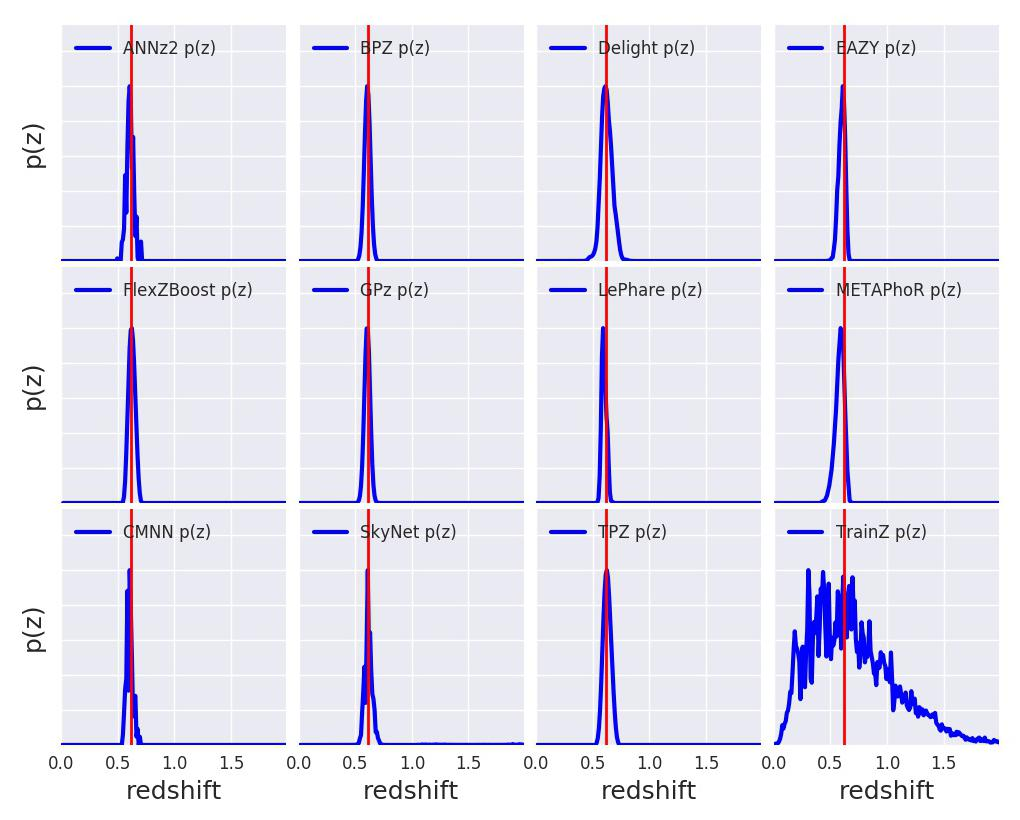
\includegraphics[width=0.49\textwidth]{fig/pz_12codes_261931_crop.jpg}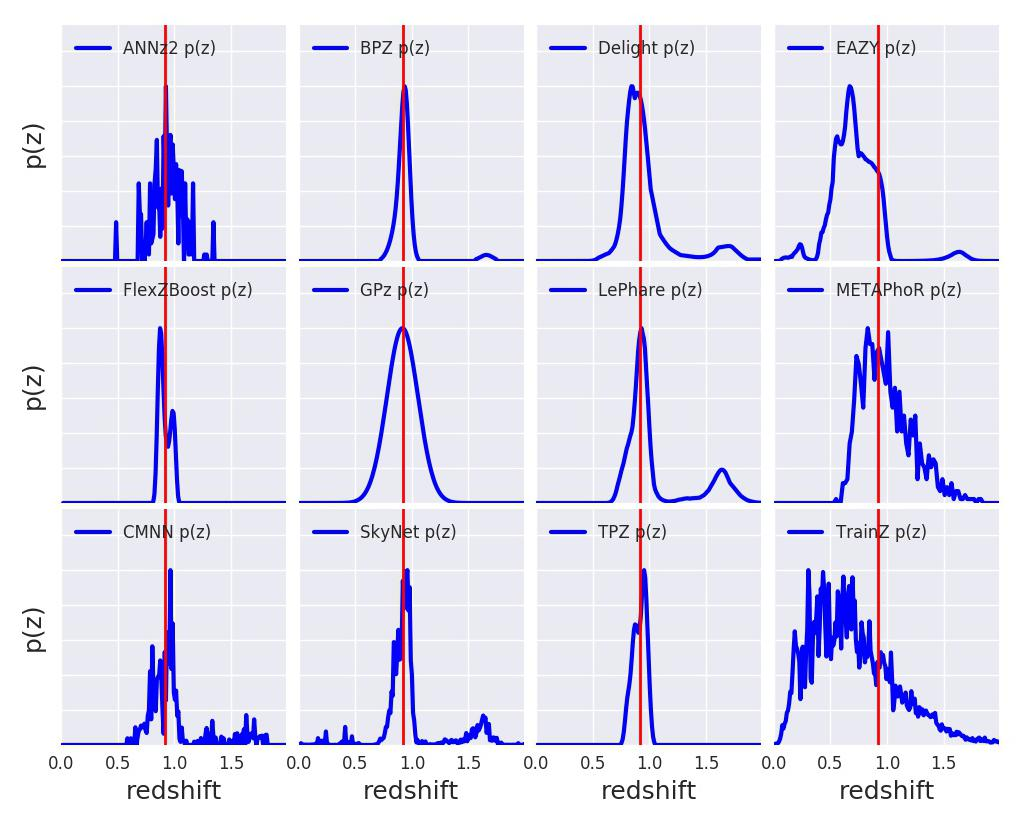
\includegraphics[width=0.5\textwidth]{fig/pz_12codes_471167_crop.jpg}\\
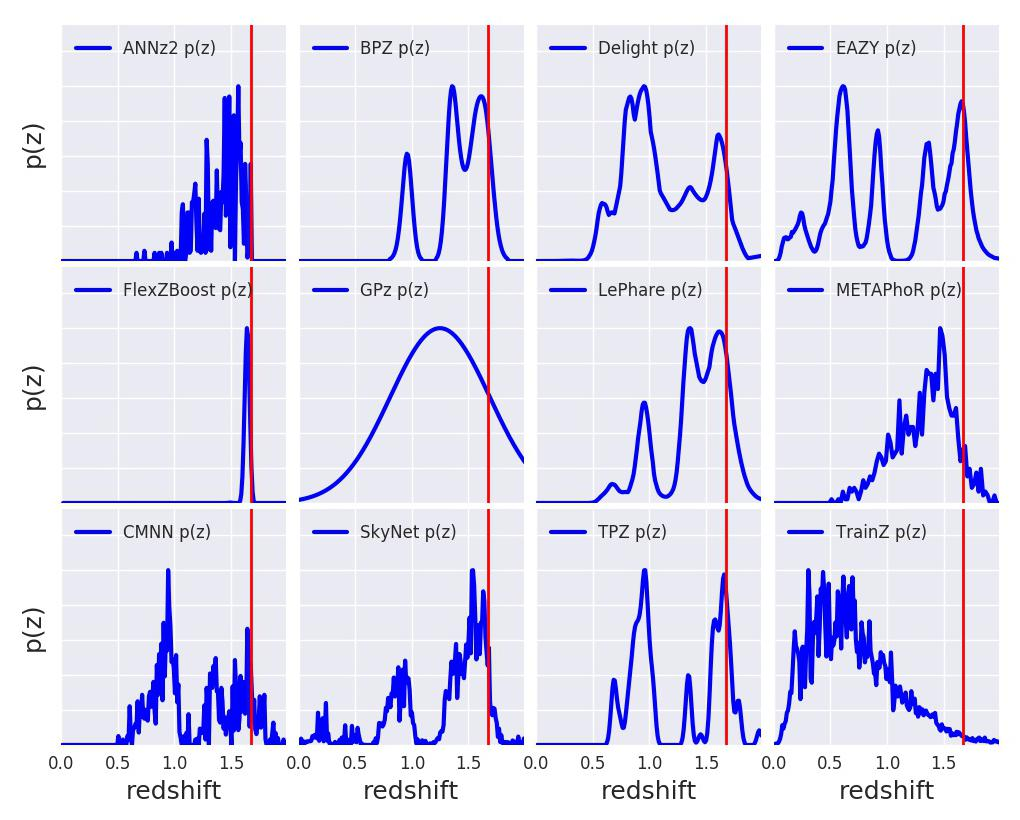
\includegraphics[width=0.49\textwidth]{fig/pz_12codes_713178_crop.jpg}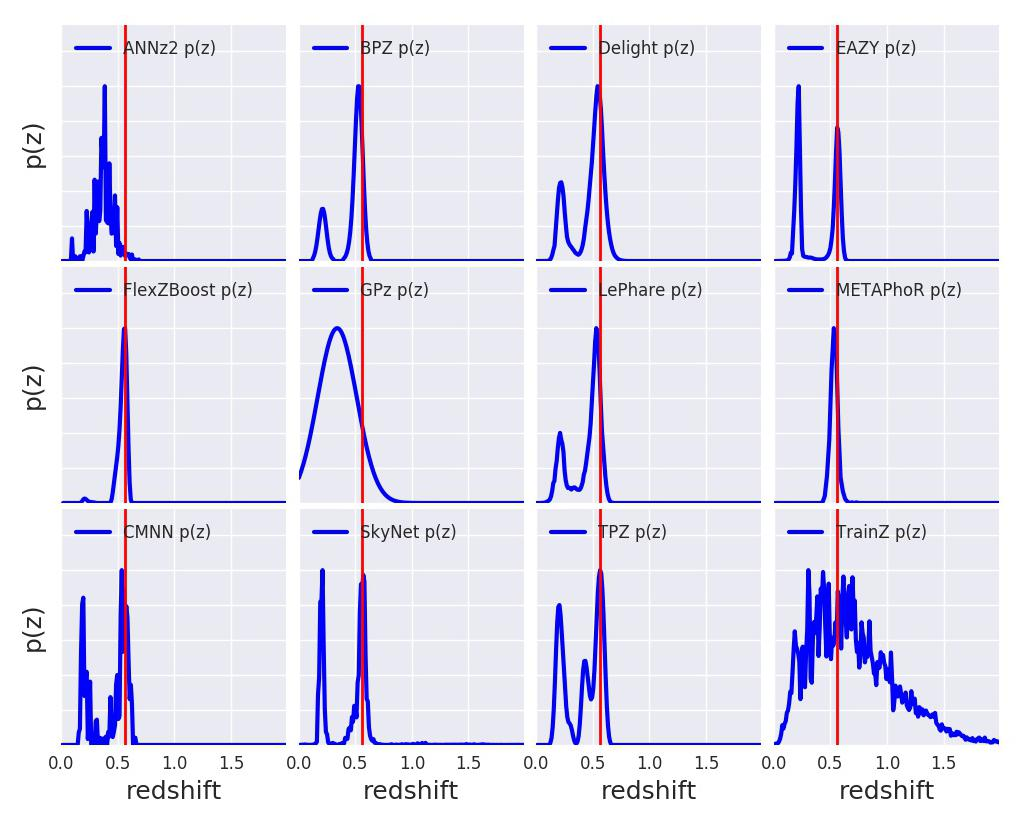
\includegraphics[width=0.49\textwidth]{fig/pz_12codes_982747_crop.jpg}
\caption{Four illustrative examples of individual p(z) distributions produced by the codes.  The red vertical line represents the true redshift.  Examples are chosen with common features seen in PDFs: tight unimodal $p(z)$ (upper left), broad unimodal $p(z)$ (upper right), bimodal $p(z)$ (lower right), and complex/multimodal $p(z)$ (lower left).  Codes show varying amounts of small-scale structure in their reconstruction of the posterior distribution.  We see varying responses from the codes in the presence of color degeneracies and photometric errors, resulting in narrow and broad unimodal, bimodal, and multi-modal $p(z)$ curves.} \label{fig:pz_examples}
\end{figure*}

%\begin{figure*}
%\centering
%\includegraphics[width=\textwidth]{fig/QQplot_11codes.jpg}
%\caption{The QQ plots produced for every photo-$z$ code.  \aim{Consider making this a plot of QQ minus that diagonal for better contrast between methods.}\red{The PIT histogram is essentially this, which is one of the main reasons to include both.  QQ is a fairly standard form, so plotting in this fashion rather than the difference seems better to me, given that we also ahve the PIT histograms. --SJS}} \label{fig:qq}
%\end{figure*}

\begin{figure*}
\centering
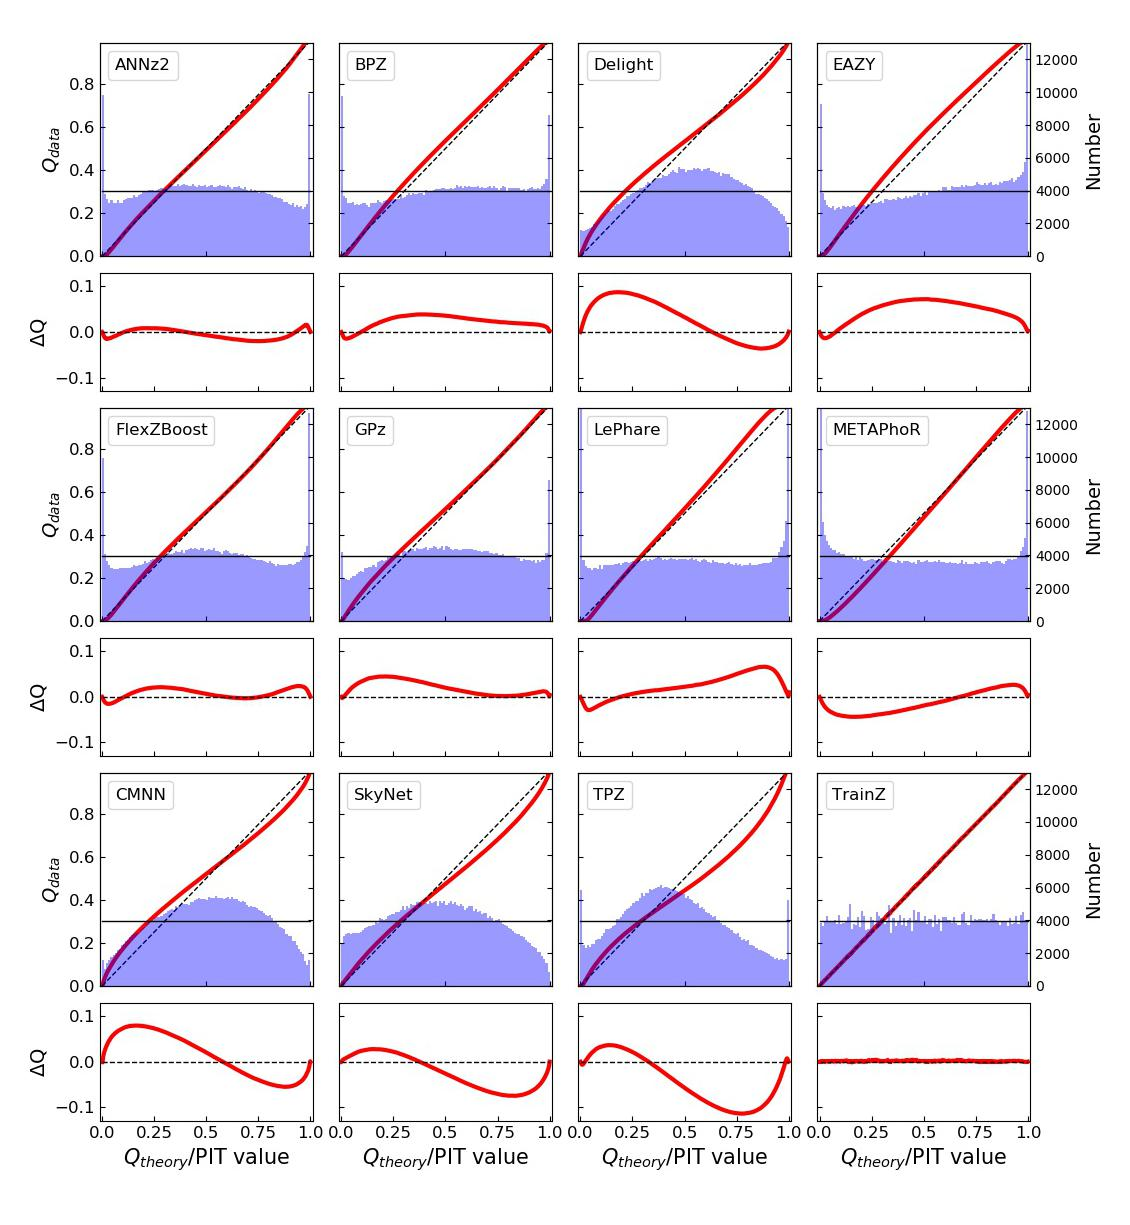
\includegraphics[width=\textwidth]{fig/PITANDQQplot_12codes_crop.jpg}
\caption{Summary plots for all twelve photo-$z$ codes illustrating performance for the interim posterior statistics. The top panel of each pair shows both the Quantile-Quantile (QQ) plot (red) and the histogram of PIT values (blue).  The desired behavior is a QQ plot that matches the diagonal dashed line, and a PIT histogram that matches a uniform distribution matching the thin horizontal black line.  The bottom panel of each pair shows the difference between the QQ quantile and the diagonal, illustrating departure from the desired performance.  Histograms with an overabundance of PIT values at the centre of the distribution indicate $p(z)$ distributions that are overly broad, while an excess of values at the extrema indicate $p(z)$ distributions that are overly narrow.  Values of PIT=0 and PIT=1 indicate ``catastrophic failures'' where the true redshift is completely outside the support of $p(z)$.  Asymmetric features are indicative of systematic bias in the redshift predictions.  A variety of behaviors are evident, and specific details are discussed in the text.}
\label{fig:pitqq}
\end{figure*}

Fig.~\ref{fig:pz_examples} Shows the $p(z)$ produced by each of our twelve photo-$z$ codes for four example galaxies which exemplify some prominent cases that arise when estimating photo-$z$ PDFs: a narrow, unimodal redshift solution, a broader unimodal solution, a bimodal distribution, and a complex, multimodal distribution.
The red vertical line represents the true redshift of the individual galaxy, and the blue curve represents the redshift probability.
Several features are obvious even in these illustrative examples.
\textsc{ANNz2, METAPhoR, NN,} and \textsc{SkyNet} all show an excess of small-scale features, which appear to be print-through of the underlying training set galaxies.  For example, in \textsc{CMNN} the $p(z)$ are a simply a weighted histogram of all spectroscopic training galaxies in nearby colour space with no smoothing applied, so the substructure is due to the finite number of neighbours, and is not unexpected.
\textsc{GPZ} (in its current implementation), on the other hand, always produces a single Gaussian, which broadens to cover the multi-modal redshift solutions seen in other codes.
%Interestingly, while \textsc{ANNz2} shows an abundance of small scale structure in individual $p(z)$ measurements (see Fig.~\ref{fig:pz_examples}), the summed $\hat{N}(z)$ is rather smooth, where the small scale features average out.  This is not the case for the two other codes that show an abundance of substructure in their individual $p(z)$: both \textsc{CMNN} and \textsc{SkyNet} show small scale features both in $p(z)$ and $\hat{N}(z)$.

As stated in Section~\ref{sec:metrics}, $p(z)$ is parameterized as $\approx 200$ piecewise constant bins covering $0<z<2$ for all twelve codes, giving a grid size of roughly $\delta z = 0.01$ for each code.
A piecewise constant grid was a natural choice for some photo-$z$ codes, for instance most template-based codes compute likelihoods on a fixed grid.
In contrast, FlexZBoost, for example, can return estimates on any grid without compression errors as it’s a basis expansion method where only the expansion coefficients need to be stored.
Codes with a native output format other than the shared piecewise constant binning scheme (or one that can be losslessly converted to it) may suffer from loss of information when converting to it, which could artificially favor some codes over others.

Furthermore, the fidelity of photo-$z$ interim posteriors in this format varies with the quality of the photometry.
For faint galaxies, this redshift resolution is sufficient to capture the shape of $p(z)$ for the majority of the test sample, where photometric errors on the faint galaxies lead to somewhat broad peaks in the redshift posterior.
However, as can be seen in e.~g.~the top left panel of Fig.~\ref{fig:pz_examples}, for bright galaxies with narrow $p(z)$ the grid spacing of $\delta z = 0.01$ is not sufficient to resolve the peak.
This is consistent with the results described in \citet[]{Malz:qp}, who find that quantiles (and, to a lesser degree, samples) often outperform gridded $p(z)$, particularly for bright objects and in the presence of harsher storage constraints.
With a full 200 numbers to capture the information of each photo-$z$ PDF, any parametrization will perform adequately, but other storage parametrizations and limits on storage resources may be considered in future work.
%Switching to a quantile based parameterization may be more costly computationally, for example template-based codes would need to test more grid point in order to resolve the quantiles for bright galaxies.  However, the computational time for template based codes scales roughly linearly with the number of grid points, so this may be a reasonable thing to implement.
We will discuss this further in Section~\ref{sec:discussion}.
% \red{someone review this statement to make sure that I'm saying this correctly!}

Fig.~\ref{fig:pitqq} shows both the quantile-quantile plots (red) and the histogram of PIT values (blue) summarizing the results from each photo-$z$ code.  The red line shows the measured quantiles, while the black diagonal represents the ideal QQ values if the distribution were perfectly reproduced.  A second panel below the main panel for each code shows the difference between $Q_{data}$ and $Q_{theory}$, i.~e.~the departure from the diagonal, for clarity.
Biases and trends in whether the average width of the $p(z)$ values being over/under-predicted are evident.  An overall bias where the predicted redshift is systematically low manifests as the measured QQ value falling above the diagonal, as is the case for \textsc{BPZ} and \textsc{EAZY}, while a systematic overprediction shows up as the measured QQ value falling below the diagonal, as seen in \textsc{TPZ}.  In terms of PIT histograms, a systematic underprediction of redshift corresponds to fewer PIT values at $PIT<0.5$ and more at $PIT>0.5$, while a systematic overprediction will show the opposite.

Examination of the PIT histograms and QQ plots shows that there are fairly generic issues with the width of $p(z)$ uncertainties: \textsc{Delight, CMNN, SkyNet} and \textsc{TPZ} all show a PIT histogram with an dearth of low values and and an excess of high values, signs that, on average, their $p(z)$ are more broad than the true distribution of redshifts.  \textsc{METAPhoR} shows the opposite trend, indicating the the $p(z)$  are more narrow than the distributions given by the true redshifts.  In all of these code cases there is a free parameter or bandwidth that can be used to tune uncertainties.  The sensitivity of multiple codes to this bandwidth choice emphasizes the fact that great care must be taken in setting user-defined parameters in photo-$z$ codes, even in the presence of representative training/validation data.  for \textsc{FlexZBoost} the ``sharpening'' parameter (described in Section~\ref{sec:flexzboost}) plays a key role in improving the results, resulting in a QQ plot that is very nearly diagonal.  A similar sharpening procedure could be beneficial for several codes.
Interestingly, the three purely template-based codes, \textsc{BPZ, EAZY}, and \textsc{LePhare}, show relatively well behaved $p(z)$ statistics (albeit with some bias), which may indicate that the likelihood estimation with representative templates is accurately capturing the uncertainties on individual redshifts.

%Fig.~\ref{fig:pitqq} shows the PIT histogram plots produced by each photo-$z$ code.
%These plots show information that is very similar to that shown in the QQ plot in many ways.
The ideal PIT histogram would follow the black dashed line, representing a uniform distribution of PIT values, equivalent to the diagonal line in the QQ plot.
Overly broad $p(z)$ values show up as an excess of PIT values near $0.5$ and a dearth of values at the edges, while overly narrow $p(z)$ will have an excess at the edges and will be missing values at the centre.
Another feature evident in the PIT histograms is the number of ``catastrophic outlier'' values where the true redshift falls outside of the non-zero support of $p(z)$, corresponding to PIT$=0.0$ or $1.0$ is more apparent than in the QQ plots.  Following Kodra \& Newman (in prep.) we define $f_{\rm O}$ as the fraction of objects with $PIT<0.0001$ or $PIT>0.9999$.  Table~\ref{tab:pitoutlier} lists these fractions for each of the codes. For a proper Uniform distribution we expect a value of $0.0002$.  Several codes show a marked excess, with \textsc{ANNz2, FlexZBoost, LePhare, and METAPhoR} with $f_{\rm O} > 0.02$, indicating a sizeable number of catastrophic redshift solutions where the true redshift is not covered by the extent of $p(z)$.  For \textsc{METAPhoR} this may be partially due to an overall underprediction of the $p(z)$ width, however this is not the case for the other codes.  \textsc{LePhare} is a particular outlier with nearly 5 per cent of objects outside of $p(z)$ support.  Further study will be necessary to determine what is causing these misclassifications for \textsc{LePhare}.  As expected, and by design, \textsc{TrainZ} has the proper fraction of outliers for the $f_{\rm O}$ statistic.


\begin{table}
\setlength{\tabcolsep}{2pt}
\centering
\caption{The fraction of ``catastrophic outlier'' PIT values.  We expect a value of 0.0002 for a proper Uniform distribution.  An excess over this small value indicates true redshifts that fall outside the non-zero support of the $p(z)$.  }\label{tab:pitoutlier}
\begin{tabular}{lc}
\hline
\hline
 ``catastrophic outlier''\\ PIT fraction\\
\hline
Photo-z Code & fraction PIT$<10^{-4}$ or $>$0.9999\\
\hline
\textsc{ANNz2} & 0.0265\\
\textsc{BPZ} & 0.0192\\
\textsc{Delight} & 0.0006\\
\textsc{EAZY} & 0.0154\\
\textsc{FlexZBoost} & 0.0202\\
\textsc{GPz} & 0.0058\\
\textsc{LePhare} & 0.0486\\
\textsc{METAPhoR}& 0.0229\\
\textsc{CMNN} & 0.0034\\
\textsc{Skynet} & 0.0001\\
\textsc{TPZ} & 0.0130\\
\hline
\textsc{TrainZ} & 0.0002\\
\end{tabular}
\end{table}


%\begin{figure*}
%\centering
%\includegraphics[width=\textwidth]{fig/PIT_histogram_plot_11codes.jpg}
%\caption{The PIT histogram plots produced for every photo-$z$ code.  Ideal behaviour would match a uniform distribution, indicated by the horizontal dashed line.  Histograms with an overabundance of PIT values at the centre of the distribution indicate $p(z)$ distributions that are overly broad, while an excess of values at the extrema indicate $p(z)$ distributions that are overly narrow.  Values of PIT=0 and PIT=1 indicate ``catastrophic failures'' where the true redshift is completely outside the support of $p(z)$.  Asymmetric features are indicative of systematic bias in the redshift predictions.
%\aim{Could we combine this with the previous figure by plotting both as differences from ideal on one plot with left and right axis labels?  The information seems degenerate (which makes sense!)}\red{as you say, the information is degenerat, this form emphasizes the differences a bit more, and shows off the catastrophic outliers with PIT=0 and 1 a bit better in my mind.} } \label{fig:pit}
%\end{figure*}
\begin{figure*}
\centering
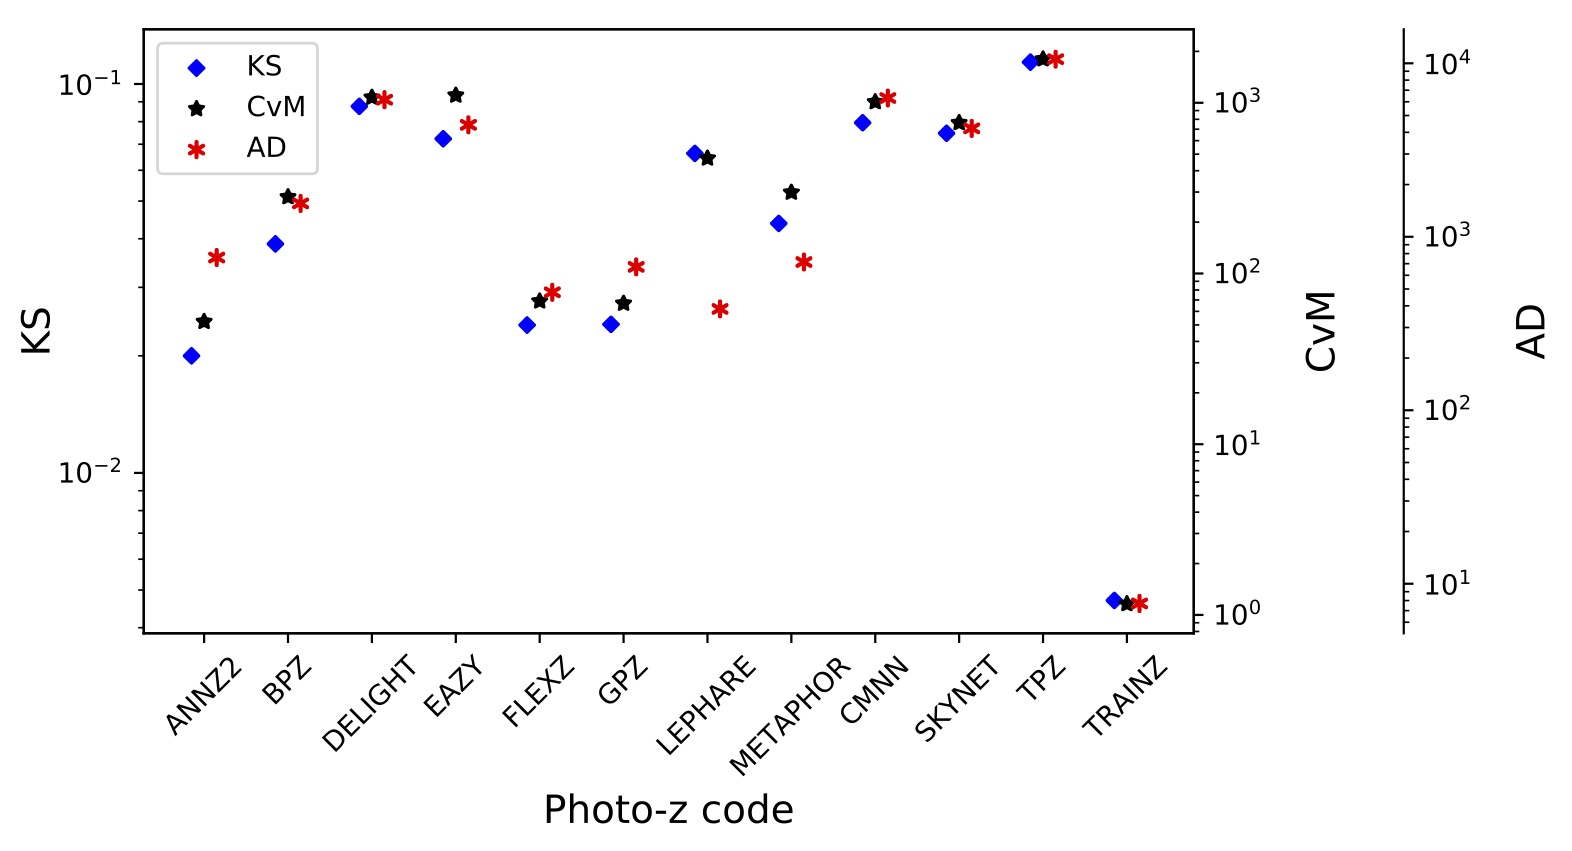
\includegraphics[width=\textwidth]{fig/KSvsCvMvsAD_PIT_withnull_jpg.jpg}
\caption{A visual representation of the Kolmogorov-Smirnoff (KS, blue diamond), Cramer-von Mises (CvM, black star), and Anderson-Darling (AD, red asterisk) statistics for the PIT distributions.  The statistics are often highly correlated, though the AD statistic truncates the extrema of the distribution and can have disparate values compared to KS and CvM.} \label{fig:pit_stats}
\end{figure*}

Fig.~\ref{fig:pit_stats} shows comparative metric values for the quantitative Kolmogorov-Smirnoff (KS), Cramer-Von Mises (CvM), and Anderson Darling (AD) test statistics for each of the codes based on comparing the distribution of their PIT values to the expected uniform distribution over the interval [0,1].  The individual values of the statistic are not as important as the comparative score between the different codes.
%\red{Can p-values be supplied for each statistic? The statistics themselves are difficult to interpret, other than ``lower is better'' (p-value in skgof was broken, having trouble finding 1-sample KS calculation for uniform distribution)}
The AD test statistic diverges for values that include the extrema, and thus is calculated by excluding the edges of the distribution.
We calculate the AD statistic over the range of PIT values $v=[0.01,0.99]$.  \textsc{ANNz2} and \textsc{FlexZBoost} score very well for the PIT metrics.
\textsc{METAPhoR} and \textsc{LePhare} score very well in the PIT AD statistic, but both have a large number of catastrophic outliers, resulting in higher KS and CvM scores.

Given the near-perfect training data, examining the individual codes for explanations for departures from the expected behaviour will be instructive in avoiding similar problems in future tests.
\textsc{ANNz2} performs quite well in $p(z)$ based metrics.  In the specific implementation employed in this paper, the final $p(z)$ is a weighted average of five neural-nets.  During the training process \textsc{ANNz2} compares the percentiles of the redshift training sample against the CDFs of the $p(z)$ sample.  Distributions that more closely match are given extra weight, and the final weights are designed to produce accurate percentiles.  Given that our metrics are focused on the percentile distributions, it is unsurprising that \textsc{ANNz2} performs well in the given metrics.  The discreteness in the individual $p(z)$ estimated by \textsc{ANNz2} can be attributed to the fact that the code was run as a classifier, assigning weights to discrete bins of redshift.  While multiple bins may receive weight, the bins themselves will still be discretized, and no additional smoothing was performed.
Overall, \textsc{FlexZBoost} and \textsc{ANNz2} show the best ensemble agreement in their distribution of PIT values.

\subsection{Metrics of the stacked estimator of the redshift distribution}\label{sec:stackedmetrics}

\begin{figure*}
\centering
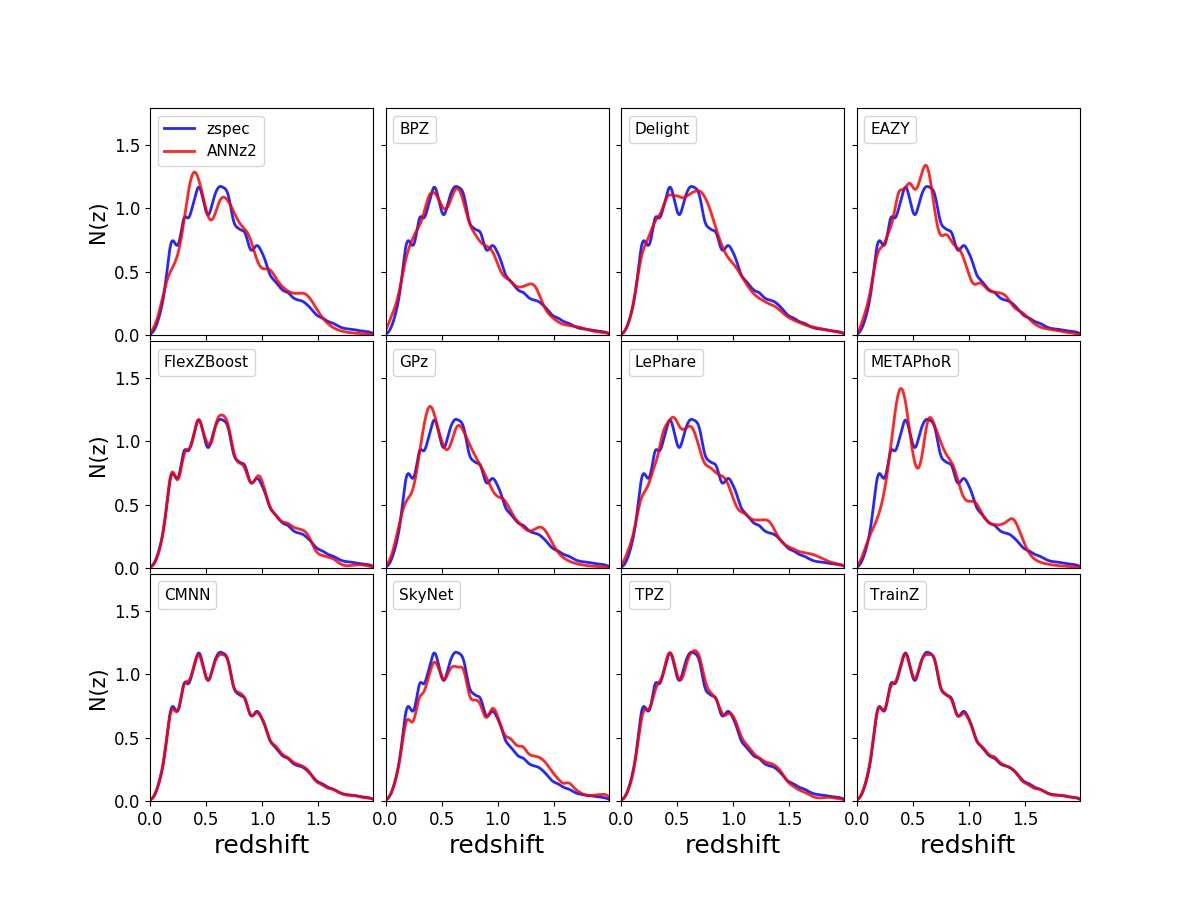
\includegraphics[width=\textwidth]{fig/NZsumplot_12codes_scottsrule.jpg}
\caption{The stacked $p(z)$ produced by each photo-$z$ code ($\hat{N}(z)$, red) compared to the spectroscopic redshift distribution ($N'(z)$, blue).  Varying levels of small-scale structure are seen in the codes.  Both $\hat{N}(z)$ and $N'(z)$ are smoothed using a single bandwidth chosen via Scott's rule for all codes.} \label{fig:nz}
%\aim{Arguably this could also be clarified by showing the true $n'(z)$ once and then differences from it for each cod's stacked estimator\dots}\scc{what if we plot the difference between true and stacked rather than soverposing the two lines? Sam please do not hate me.}
\end{figure*}

\begin{figure*}
\centering
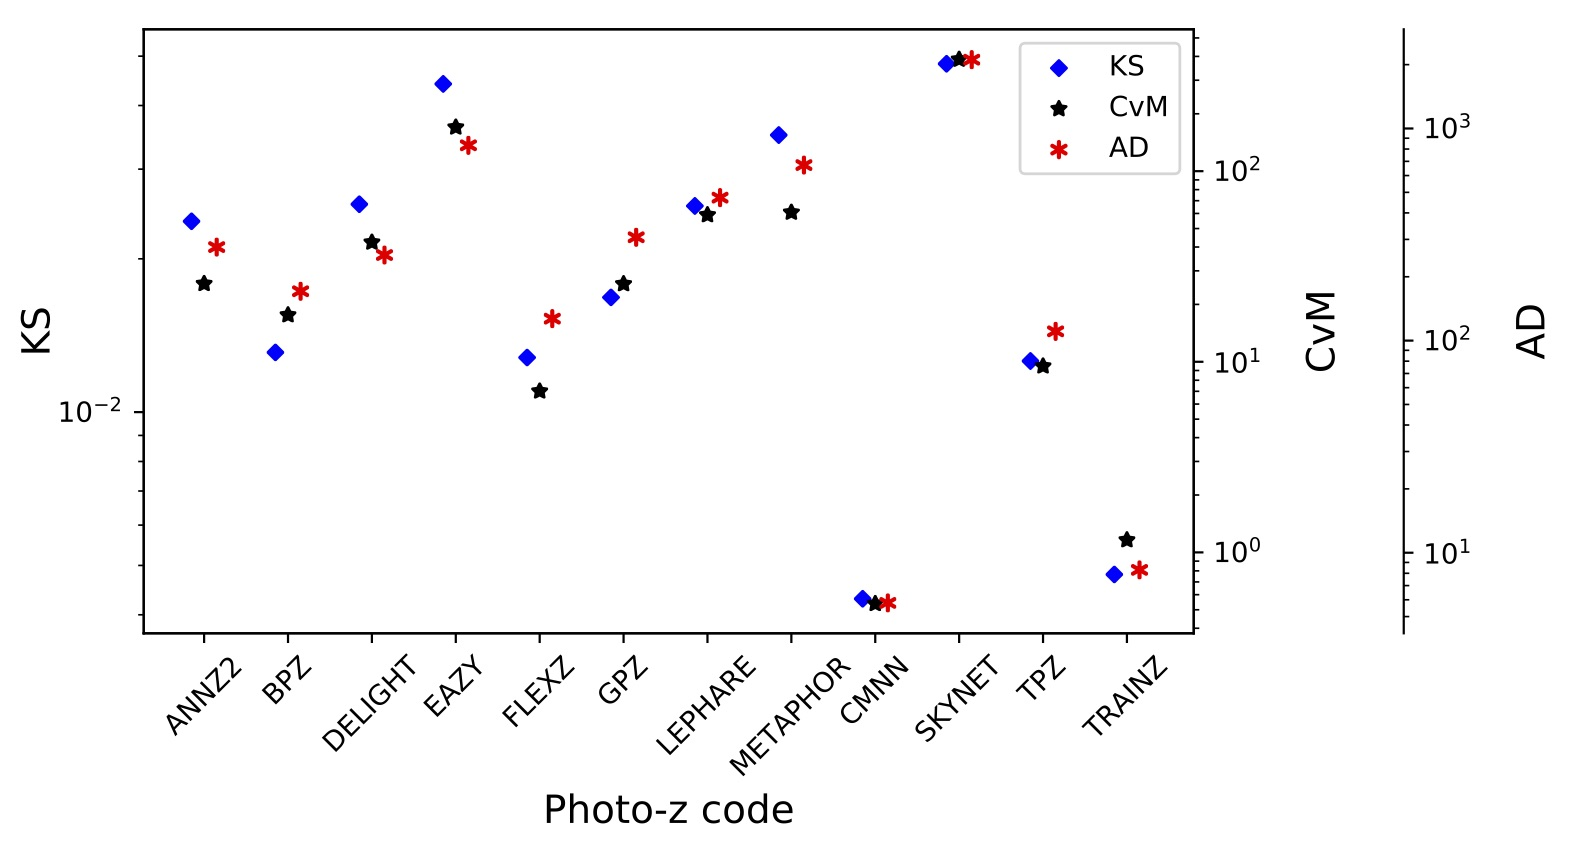
\includegraphics[width=\textwidth]{fig/KSvsCvMvsAD_NZ_withnull_jpg.jpg}
\caption{A visual representation of the Kolmogorov-Smirnoff (KS, blue diamond), Cramer-von Mises (CvM, black star), and Anderson-Darling (AD, red asterisk) statistics for the $\hat{N}(z)$ distributions. The statistics are correlated, the codes with the lowest KS statistics tend to have the lowest CvM and AD statistics.  \textsc{CMNN} performs markedly better than the others in reconstructing the overall $N(z)$ distribution, while \textsc{SkyNet} scores poorly due to an overall bias in its redshift predictions.} \label{fig:nz_stats}
\end{figure*}

Fig.~\ref{fig:nz} shows the stacked $\hat{N}(z)$ distribution compared to the true redshift distribution $N'(z)$ for all tested codes.  The red line indicates the summed $p(z)$ for each code, while the blue line shows the true redshift distribution. All distributions are smoothed via kernel density estimation (KDE) with a common bandwidth chosen via Scott's rule \citep{Scott:1992} in order to minimize differences in small-scale features and make for a more uniform comparison between codes.  While Scott's rule is used to display $N'(z)$ in the figure, all quantitative statistics are computed via the empirical CDF, and are thus unaffected by bandwidth/smoothing choice.
%New text for the new figure
As expected, \textsc{TrainZ} is in excellent agreement with the true redshift distribution: as the training sample is selected from the same underlying distribution as the test set, the redshift distributions are identical, up to Poisson fluctuations due to the finite number of sample galaxies.  \textsc{CMNN} is also in excellent agreement for similar reasons: with a representative training sample of galaxies spanning the colour-space, the sum of the colour-matched neighbour redshifts should return the true redshift distribution. \textsc{FlexZBoost} and \textsc{TPZ} also show very good agreement, with only slight departures, with an over/under-prediction in the high redshift tail of $\hat{N}(z)$ evident around $z\sim1.4$.  In fact, several of the other codes show an excess at $z \sim 1.4$, particularly the template-based codes \textsc{BPZ}, \textsc{EAZY}, and \textsc{LePhare}.  This is likely due to the $4000\ {\rm \AA}$ break passing through the gap between the $z$ and $y$ filters, resulting in a drastic change in $z-y$ colour for galaxies in this redshift range.  With a relative dearth of strong features blue-ward of the $4000\ {\rm \AA}$ break in most galaxy SEDs, the colour change in the two reddest filter bandpasses of a survey has a large influence on the redshift determination.  The $z\sim1.4$ feature is one of the most prominent sources of larger uncertainty in individual galaxy $p(z)$.
In our sample individual galaxy $p(z)$'s tend to be broader around $z\sim1.4$ and point estimates are more uncertain in this regime, as is readily seen in the point-estimate plots shown in Fig.~\ref{fig:pz_pointestimates} and described in the Appendix.  This feature is not unique to this dataset, it is a common occurrence in photo-$z$ estimation.  The fact that similar excesses appear in Figure~\ref{fig:nz} for \textsc{ANNz2} and \textsc{METAPhoR} shows that the effect is not limited to template-based codes.  However, the lack of such a feature in the other codes shows that it is possible to eliminate the degeneracies.  Further study on this issue may provide a solution for codes that suffer from this shortcoming.

%end of new text (and slightly modified text)
Two of the machine learning based codes, \textsc{ANNz2} and \textsc{METAPhoR}, appear to be over-trained, adding excess galaxy probability to the redshift peaks with the largest number of training galaxies, and missing probability in the troughs where training galaxies are of fewer number.
Given that our training data is drawn from the same galaxy population as the test set, and our data has prominent peaks in $N'(z)$, perhaps it is not unexpected that such overtraining occurs in some codes, though the fact that it does not occur in all training-based codes indicates that it may be due to specifics of the implementations of \textsc{ANNz2} and \textsc{METAPhoR}.
A more extensive training/validation set might allow for a better choice of smoothing parameters in individual codes that would avoid such overtraining for these particular codes.
%\aim{Move the text on Scott's Rule to Discussion?}
%Scott's rule \citep{Scott:1992} was used to determine the smoothing bandwidth of the true redshift sample: that is, a single smoothing scale was chosen to represent the true redshift sample for all twelve codes.
%As with the $p(z)$ values in Figure~\ref{fig:pitqq}, different levels of substructure are obvious for the different codes.
%While Scott's rule provides a relatively good general smoothing scale to represent the true $N'(z)$, there are smaller scale fluctuations: while \textsc{FlexZBoost} and \textsc{CMNN} appear somewhat discrepant in Fig.~\ref{fig:nz}, they are actually the two most accurate in terms of their quantitative measurements.
%\textsc{SkyNet} also shows excess small-scale structure, but also shows significant overestimate of the high redshift galaxy population.
\textsc{SkyNet} shows an obvious redshift bias, evident both visually in Figure~\ref{fig:nz} and in the first moment of N(z) listed in Table~\ref{tab:moments}, where it is clearly an outlier.  \textsc{SkyNet} employed a method where a random sample of training galaxies was chosen, but there was no test that the subset was completely representative of the overall redshift distribution.  Unlike the previous implementation of \textsc{SkyNet} in \citet{Bonnett:15}, no effort was made to add extra weight to more rare low and high redshift galaxies.  Either of these decisions could be the cause of the bias seen in our results.  Future runs of \textsc{SkyNet} will explore these implementation choices and their effects.


Figure~\ref{fig:nz_stats} shows the quantitative Kolmogorov-Smirnoff (KS), Cramer-Von Mises (CvM), and Anderson Darling (AD) test statistics for each of the codes for the $\hat{N}(z)$ based measures.
%\red{Can p-values be supplied for each statistic? The statistics themselves are difficult to interpret, other than ``lower is better'' (no, p-values are very difficult to compute for non-uniform distributions)}
\textsc{FlexZBoost}, \textsc{CMNN}, and \textsc{TPZ} outperform the other codes in the $\hat{N}(z)$ metrics.
It is unsurprising that \textsc{CMNN} scores well, as with a near perfectly representative training set means that choosing neighbouring points in color/magnitude space should lead to excellent agreement in the final $\hat{N}(z)$ estimate.  \textsc{TPZ} performed quite poorly in $p(z)$ statistics, but results in a good fit to the overall $N(z)$.  This is somewhat surprising, as performance was optimized for accurate $p(z)$, not $\hat{N}(z)$.  During the validation stage for \textsc{TPZ}, there was a trade off between the width of the $p(z)$ when adjusting a smoothing parameter and overall redshift bias.  The optimal result in the PIT metrics, as illustrated in the shape of the QQ plot, does contain some level of bias as well as a slight underprediction of mean $p(z)$ width, which translates to poor metric scores.  This is something that will be looked into for \textsc{TPZ} in the future.

%\red{discussion of why NN and FZBoost are doing well, how we can try to improve the other codes}
%\textcolor{cyan}{Ann: }


Table~\ref{tab:cdeloss} shows the CDE loss statistic for each photo-$z$ code.  Once again \textsc{FlexZBoost} and \textsc{CMNN} score very well for the stacked $\hat{N}(z)$ metrics, as do \textsc{GPz} and \textsc{TPZ}.  The CDE loss measures how well individual PDFs are estimated, and codes with a low CDE loss tend to have good $\hat{N}(z)$ estimates (though the reverse is not necessarily true). \textsc{FlexZBoost} is optimized to minimize CDE loss which may explain why the method has good ensemble metrics as well. Note from Table~\ref{tab:cdeloss} that both \textsc{FlexZBoost} and \textsc{CMNN} have low CDE losses.  Empirically, we have found that PIT RMSE is not as closely correlated to CDE loss as it is to the $N(z)$ statistics.  As CDE loss is a better measure of individual redshift performance, rather than ensemble distribution performance, this statistic is a better indicator of which codes will be most likely to perform well for science cases where single objects are employed.

Table~\ref{tab:rmse} gives the root-mean-square-error (RMSE) statistics for both the PIT and N(z) estimators.  The PIT value calculates the RMSE between the quantiles shown in the QQ plot in Figure~\ref{fig:pitqq} and the diagonal, while the N(z) calculates the RMSE between the cumulative distribution of the stacked $\hat{N}(z)$ and the true redshift distribution $N'(z)$.  %\red{more about RMSE?  Or remove it? It's barely described in Section~\ref{sec:metrics} and wasn't even referred to in the text until I added this on June 29th--SJS.}

Table~\ref{tab:moments} lists the first three moments of the stacked $\hat{N}(z)$ distribution, including the moments of the ``truth'' distribution for comparison.  Several codes are able to reproduce the mean and variance of the distribution to less than a per cent, while several codes do not, which may be a cause for concern, given that mean and variance of the redshift distribution are key properties in cosmological analyses.  We note that this stated goal of the study as defined for participants was to accurately reproduce $p(z)$, the ``stacking'' of the probability distributions to estimate $\hat{N}(z)$ was not the focus as stated to the participants.  This explains why some of the best-performing empirical codes in terms of $p(z)$ measures (e.~g.~\textsc{FlexZBoost}) do not do as well at reproducing $\hat{N}(z)$ moments.  Had we defined a different parameter to optimize, in this case overall accuracy of $\hat{N}(z)$ rather than individual $p(z)$, would result in improved performance in a particular metric.  That is, optimizing photo-$z$ performance for one metric does not automatically give optimal performance for other metrics.  As previously stated, there are a variety of scientific use cases for photo-$z$'s in large upcoming surveys, and care must be taken in how the metrics used to optimize catalog photometric redshifts are defined as well as in how they are used.  In addition, very few scientific use cases will employ the overall $\hat{N}(z)$ with no cuts, as we explore in this paper.  We discuss more realistic tomographic bin selections that will be explored in a follow-up paper in Section~\ref{sec:futurework}.
%\red{[mention that we are calculating moments for the entire sample, will look at fiducial tomographic bins in a follow-up paper (unless group and reviewers realy think we should include in this paper.]}
%\red{FlexZBoost has some of the best $n(z)$ statistics, but the moments are not good.  Why is this?  Is it the over/underprediction of the high redshift part of the distribution?  Discuss this after talking with Rafael.}

%\subsection{Response of Individual Codes}
%\label{sec:res:pz_indiv_codes}
%\red{this may be incorporated in to 5.1 and 5.2 rather than live in its own section!}


%\red{HOW CODES deal with negative fluxes, and magnitude uncertainties}

%\red{overall conclusions of the Results section}

\subsection{Interpretation of metrics}\label{sec:caution}
%Caution on metrics and photo-$z$ codes}\label{sec:caution}
%(Alex Malz, Sam Schmidt)

Samples from accurate photo-$z$ posteriors should reproduce the space of $p(z, data)$. However, it is difficult to test this reconstruction given our data set, as the galaxy distributions arise from mock objects pasted on to an underlying dark matter halo catalogue with properties designed to match empirical relations, rather than being drawn from statistical distributions in redshift.  In previous sections we have mentioned that optimizing for a specific metric does not guarantee good performance on other metrics, nor is there any guarantee that good performance by our metrics corresponds to \textit{accurate} photo-$z$ posteriors.
%\aim{Explain that samples from accurate photo-$z$ posteriors should reconstruct the space of $p(z, data)$, a test we can't check with our datasets.}
In other words, we can construct photo-$z$ estimators that provide good coverage in many of our tests, but which have very little predictive power.


The \trainz\ estimator, which assigns every galaxy a $p(z)$ equal to $N(z)$ of the training set as described in Section~\ref{sec:method:trainz}, is introduced as a ``null test'' to demonstrate this point via \textit{reductio ad absurdum}.
\trainz\ outperforms all codes on the PIT-based metrics, and all but one code on the $N(z)$ based statistics.
Because our training set is perfectly representative of the test set, $N(z)$ should be identical for both sets down to statistical noise.
%\textit{Explain the connection between \trainz\ and these metrics.}

The CDE loss and point estimate metrics, however, successfully identify problems with \trainz.
As shown in Appendix~\ref{sec:pointmetrics}, \trainz has identical $ZPEAK$ and $ZWEIGHT$ values for every galaxy, and thus the photo-$z$s are constant as a function of spec-$z$s, i.e. a horizontal line at the mode and mean of the training set distribution respectively.  The explicit dependence on the \it{individual} posteriors in the calculation of the CDE loss, described in Section~\ref{sec:CDE_loss}, distinguishes this metric from the other $p(z)$ metrics that test the overall ensemble of $p(z)$ distributions.  With a representative training set, \trainz\ will score well on the ensemble metrics, but fails miserably for metrics tied to individual redshifts.  We note that many of the ensemble-based metrics are prominent in the photo-$z$ literature despite their inability to identify problems such as those exemplified by \trainz.

%\aim{Explain why CDE loss is different from other metrics (isn't fooled by \trainz) and note that the others have more of a presence in the literature despite their flaw of failing to identify this severe problem.}

% While looking at one, or even most of our metrics would have given the impression that this estimator was nearly optimal, red flags in CDE loss and point estimates reveal the problems.
%[more caution on over-reliance on metrics, and making sure that metrics test all of what you want] \red{this definitely still needs work}
In summary, context is crucial to interpreting metrics and defending against the likes of \trainz.
The best photo-$z$ method is the one that most effectively achieves our science goals, not the one that performs best on a metric that does not accurately reflect those goals.
In the absence of clear goals or the information necessary for a principled metric definition, we must think carefully before choosing a single metric

%\begin{table*}  %%% DATA TABLE %%%
%\caption{KS, CvM and AD statistics for each photo-$z$ code.} \label{tab:results}
%PIT statistic
%
%\begin{tabular}{lrrrr}
%\hline
%\bf Photo-$z$ Code & \bf KS & \bf CvM & \bf AD & \bf AD \\
%                   &        &         & $v=[0.05,0.95]$ & $v=[0.01,0.99]$        \\
%\hline
%\textsc{ANNz2} 		& $0.0200$ &   $52.25$ &   $583.0$ &   $759.2$ \\
%\textsc{BPZ} 		& $0.0388$ &  $280.79$ &  $1361.4$ &  $1557.5$ \\
%%\textsc{Delight} 	& $0.1380$ & $3040.59$ & $13880.2$ & $17761.4$ \\
%\textsc{Delight}    & $0.0876$ & $1075.17$ & $4407.8$  & $6167.5$\\
%%\textsc{EAZY} 		& $0.0690$ &  $994.19$ &  $3479.5$ &  $4158.8$ \\
%\textsc{EAZY}       & $0.0723$ & $1105.58$ & $3475.0$  & $4418.6$\\
%%\textsc{FlexZBoost} & $0.0260$ &   $70.58$ &   $595.0$ &   $533.0$ \\
%\textsc{FlexZBoost} & $0.0240$ &   $68.83$ &   $567.9$ &   $478.8$\\
%\textsc{GPz} 		& $0.0449$ &  $258.56$ &   $904.8$ &  $1414.8$ \\
%\textsc{LePhare} 	& $0.0663$ &  $473.05$ &    $85.9$ &   $383.8$ \\
%\textsc{METAPhoR} 	& $0.0438$ &  $298.56$ &   $248.6$ &   $715.5$ \\
%%\textsc{CMNN} 		& $-$ & $-$ & $-$ & $-$ \\
%\textsc{CMNN}         & $0.0795$  &$1011.11$ &  $3908.2$ &  $6307.5$ \\
%\textsc{SkyNet} 	& $0.0747$ &  $763.00$ &  $2740.2$ &  $4216.4$ \\
%\textsc{TPZ} 		& $0.1138$ & $1801.74$ &  $9046.2$ & $10565.7$ \\
%%\textsc{Frankenz}	& $-$ & $-$ & $-$ & $-$ \\
%\hline
%\end{tabular}

%Stacked $n(z)$ statistic
%
%\begin{tabular}{lrrrr}
%\hline
%\bf Photo-$z$ Code & \bf KS & \bf CvM & \bf AD & \bf AD \\
%                   &        &         & $z=[0.002,2.0]$ & $z=[0.0,2.0]$        \\
%\hline
%\textsc{ANNz2} 		& $0.0237$ &  $25.676$ &   $276.4$ &   $276.0$ \\
%\textsc{BPZ} 		& $0.0131$ &  $17.587$ &   $169.0$ &   $170.9$ \\
%%\textsc{Delight} 	& $0.0184$ &  $18.975$ &   $151.5$ &   $151.5$ \\
%\textsc{Delight}    & $0.0256$ &  $42.341$ &   $253.3$ &   $253.2$ \\
%%\textsc{EAZY} 		& $0.0434$ & $167.329$ &   $811.3$ &   $817.0$ \\
%\textsc{EAZY}       & $0.0441$ & $169.977$ &   $827.7$ &   $833.3$ \\
%%\textsc{FlexZBoost} & $0.0065$ &   $2.764$ &    $24.7$ &    $24.6$ \\
%\textsc{FlexZBoost} & $0.0128$ &   $7.007$ &  $127.02$ &   $126.9$\\
%\textsc{GPz} 		& $0.0168$ &  $25.605$ &   $307.1$ &   $307.1$ \\
%\textsc{LePhare} 	& $0.0254$ &  $58.900$ &   $477.4$ &   $472.0$ \\
%\textsc{METAPhoR} 	& $0.0350$ &  $60.790$ &   $671.9$ &   $672.3$ \\
%%\textsc{CMNN} 		& $-$ & $-$ & $-$ & $-$ \\
%\textsc{CMNN}         & $0.0043$ & $0.538$   &   $5.6$   &      $5.8$ \\
%\textsc{SkyNet} 	& $0.0483$ & $385.830$ &  $2119.4$ &  $2110.3$ \\
%\textsc{TPZ} 		& $0.0126$ &   $9.483$ &   $110.7$ &   $110.6$ \\
%%\textsc{Frankenz}	& $-$ & $-$ & $-$ & $-$ \\
%\hline
%\end{tabular}
%\end{table*}

\begin{table}  %%% DATA TABLE %%%
\centering
\caption{CDE loss statistic for each photo-$z$ code.} \label{tab:cdeloss}
\begin{tabular}{lr}
\hline
\bf Photo-$z$ Code & \bf CDE Loss \\
\hline
\textsc{ANNz2} 		& $-6.88$ \\
\textsc{BPZ} 		& $-7.82$ \\
%\textsc{Delight} 	& $-4.06$ \\
\textsc{Delight}    & $-8.33$\\
%\textsc{EAZY} 		& $-7.97$ \\
\textsc{EAZY}       & $-7.07$ \\
%\textsc{FlexZBoost} & $-11.51$ \\
\textsc{FlexZBoost} & $-10.60$\\
\textsc{GPz} 		& $-9.93$ \\
\textsc{LePhare} 	& $-1.66$ \\
\textsc{METAPhoR} 	& $-6.28$ \\
%\textsc{CMNN} 		& $-$ \\
\textsc{CMNN}         & $-10.43$ \\
\textsc{SkyNet} 	& $-7.89$ \\
\textsc{TPZ} 		& $-9.55$ \\
\hline
\trainz		& $-0.83$ \\
%\textsc{Frankenz}	& $-$  \\
%\hline
\end{tabular}
\end{table}

\begin{table}
\setlength{\tabcolsep}{2pt}
\begin{center}
\caption{Root-Mean-Square-Error (RMSE) statistics for the twelve photo-z codes for both PIT and $\hat{N}(z)$ distributions.}\label{tab:rmse}
\begin{tabular}{lcc}
\hline
\hline
Root-Mean-Square-Error \\
(RMSE) statistics \\
\hline
Photo-z Code & PIT RMSE & N(z) RMSE\\
\hline
\textsc{ANNz2}      & 0.019 & 0.0054\\
\textsc{BPZ}        & 0.032 & 0.0050\\
\textsc{Delight}    & 0.111 & 0.0056\\
\textsc{EAZY}       & 0.054 & 0.0102\\
\textsc{FlexZBoost} & 0.021 & 0.0022\\
\textsc{GPz}        & 0.027 & 0.0042\\
\textsc{LePhare}    & 0.028 & 0.0062\\
\textsc{METAPhoR}   & 0.064 & 0.0081\\
\textsc{CMNN}         & 0.108 & 0.0009\\
\textsc{Skynet}     & 0.054 & 0.0144\\
\textsc{TPZ}        & 0.082 & 0.0031\\
\hline
\trainz		& 0.0025 & 0.0013\\
\end{tabular}
\end{center}
\end{table}

%\begin{table}
%\begin{center}
%caption{RMSE Statistics for the 11 Photo-z codes for DC1 $i<25.3$ ``gold'' sample}\label{tab:pitrmse}
%%\begin{tabular}{|l|c|c|c|c|}
%\begin{tabular}{lc}
%\hline
%\hline
% PIT RMSE statistics \\
%\hline
%Photo-z Code & PIT RMSE\\
%\hline
%\texttt{ANNz2}      & 0.019\\
%\texttt{BPZ}        & 0.032\\
%\texttt{Delight}    & 0.111\\
%\texttt{EAZY}       & 0.054\\
%\texttt{FlexZBoost} & 0.021\\
%\texttt{GPz}        & 0.048\\
%texttt{LePhare}    & 0.028\\
%\texttt{METAPhoR}   & 0.064\\
%\texttt{NN}         & 0.108 \\
%\texttt{Skynet}     & 0.054\\
%texttt{TPZ}        & 0.082\\
%\hline
%\end{tabular}
%\end{center}
%\end{table}
%
%\begin{table}
%\begin{center}
%\caption{RMSE Statistics for the 11 Photo-z codes for DC1 $i<25.3$ ``gold'' sample}\label{tab:nzrmse}
%%\begin{tabular}{|l|c|c|c|c|}
%\begin{tabular}{lc}
%\hline
%\hline
% N(z) RMSE statistics \\
%\hline
%hoto-z Code & N(z) RMSE\\
%\hline
%\texttt{ANNz2}      & 0.0054\\
%\texttt{BPZ}        & 0.0050\\
%\texttt{Delight}    & 0.0056\\
%\texttt{EAZY}       & 0.0102\\
%\texttt{FlexZBoost} & 0.0022\\
%\texttt{GPz}        & 0.0042\\
%\texttt{LePhare}    & 0.0062\\
%\texttt{METAPhoR}   & 0.0081\\
%\texttt{NN}         & 0.0009\\
%\texttt{Skynet}     & 0.0144\\
%\texttt{TPZ}        & 0.0031\\
%\end{tabular}
%\end{center}
%\end{table}

\begin{table}
\setlength{\tabcolsep}{2pt}
\caption{Moments of the stacked $\hat{N}(z)$ distribution}\label{tab:moments}
\begin{tabular}{lccc}
\hline
\hline
 \multicolumn{4}{l}{Stacked $n(z)$ Moments} \\
\hline
              & 1st Moment & 2nd Moment & 3rd Moment \\
\textsc{Truth}     & 0.701      &   0.630    & 0.671  \\
\hline
Photo-z Code       & 1st Moment & 2nd Moment & 3rd Moment\\
\hline
\textsc{ANNz2}     & 0.702      & 0.625      & 0.653    \\
\textsc{BPZ}       & 0.699      & 0.629      & 0.671    \\
\textsc{Delight}   & 0.692      & 0.609      & 0.638    \\
\textsc{EAZY}      & 0.681      & 0.595      & 0.619    \\
\textsc{FlexZBoost}& 0.694      & 0.610      & 0.631    \\
\textsc{GPz}       & 0.696      & 0.615      & 0.639    \\
\textsc{LePhare}   & 0.718      & 0.668      & 0.741    \\
\textsc{METAPhoR}  & 0.705      & 0.628      & 0.657    \\
\textsc{CMNN}        & 0.701      & 0.628      & 0.667    \\
\textsc{Skynet}    & 0.743      & 0.708      & 0.797    \\
\textsc{TPZ}       & 0.700      & 0.619      & 0.643    \\
\hline
\trainz	   & 0.699 		& 0.627 	& 0.666 \\
\end{tabular}
\end{table}


\section{Discussion and future work}
\label{sec:discussion}
%(Sam Schmidt, Ofer Lahav, Jeff Newman, Alex Malz, Eve Kovacs, Tony Tyson, Tina Peters)

% If methods can not reach the goals on idealized data, then they will almost surely not meet those same goals when the more complex problems that we expect to arise from real LSST data are included.
% The results presented in this paper enable an evaluation of which algorithms are the most promising moving forward, and potentially point to avenues for improvement.

In contrast with other \pzpdf\ comparison papers that have aimed to identify the ``best'' code for a given survey, we have focused on the somewhat more philosophical questions of how to assess \pzpdf\ methods and how to interpret differences between codes in terms of \pzpdf\ performance.
In Section~\ref{sec:caution}, we reframe the strong performance of our pathological \pzpdf\ technique, \trainz, as a cautionary tale about the importance of choosing appropriate comparison metrics.
In Section~\ref{sec:futureexperiments}, we outline the experiments we intend to build upon this study
In Section~\ref{sec:futuredata}, we discuss the enhancements of the mock data set that will be necessary to enable the future experiments.

\subsection{Interpretation of metrics}
\label{sec:caution}
%(Alex Malz, Sam Schmidt)

We remind the reader that contributed codes were given a goal of obtaining accurate \pzpdf s, not an accurate stacked estimator of the redshift distribution, so we do not expect the same codes to necessarily perform well for both classes of metrics.
Indeed, the codes were optimized for their interpretation of our request for ``accurate \pzpdf s,'' and we expect that the implementations would have been adjusted had we requested optimization of the traditional metrics of Appendices~\ref{sec:moments} and~\ref{sec:pointmetrics}.

Furthermore, our metrics are not necessarily able to assess the fidelity of individual \pzpdf s relative to true posteriors: in the absence of a ``true PDF'' from which redshifts are drawn, it is difficult to construct metrics to measure performance for individual galaxies rather than ensembles.
(The CDE Loss metric of section~\ref{sec:CDE_loss} is an exception to this rule.)
A lack of appropriate metrics more sophisticated than the CDE Loss remains an open issue for science cases requiring accurate individual galaxy PDFs.
The metric-specific performance demonstrated in this paper implies that we may need multiple \pzpdf\ approaches tuned to each metric in order to maximize returns over all science cases in large upcoming surveys.

The \trainz\ estimator of Section~\ref{sec:trainz}, which assigns every galaxy a \pzpdf\ equal to $N(z)$ of the training set, is introduced as an experimental control or null test to demonstrate this point via \textit{reductio ad absurdum}.
Because our training set is perfectly representative of the test set, $N(z)$ should be identical for both sets down to statistical noise.
\textit{We make the alarming observation that \trainz\ outperforms all codes on the PIT-based metrics, and all but one code on the $N(z)$ based statistics.}
%\textit{Explain the connection between \trainz\ and these metrics.}

The CDE loss and point estimate metrics appropriately penalize \trainz's naivete.
As shown in Appendix~\ref{sec:pointmetrics}, \trainz ~has identical $ZPEAK$ and $ZWEIGHT$ values for every galaxy, and thus the \pz\ point estimats are constant as a function of true redshift, i.~e.~a horizontal line at the mode and mean of the training set distribution respectively.
The explicit dependence on the individual posteriors in the calculation of the CDE loss, described in Section~\ref{sec:cdelossresults}, distinguishes this metric from those of the \pzpdf\ ensemble and stacked estimator of the redshift distribution, despite their prevalence in the \pz\ literature.

% While looking at one, or even most of our metrics would have given the impression that this estimator was nearly optimal, red flags in CDE loss and point estimates reveal the problems.
%[more caution on over-reliance on metrics, and making sure that metrics test all of what you want] \red{this definitely still needs work}
In summary, context is crucial to defending against deceptively strong performers such as \trainz; \textbf{the best \pzpdf\ method is the one that most effectively achieves our science goals}, not the one that performs best on a metric that does not reflect those goals.
In the absence of a single scientific motivation or the information necessary for a principled metric definition, we must consider many metrics and be critical of the information transmitted by each.
% As stated earlier, science applications may be sensitive to individual \pzpdf s, \pzpdf\ ensembles, \pz\ point estimates, or science-specific statistics like $\hat{N}(z)$.
% We must be aware of that the optimal method for one is not necessarily optimal for the other, and in fact several photo-$z$ algorithms may be necessary in the final cosmological analysis in order to satisfy the requirements of all science use cases.
% The example of the simple \trainz\ estimator described in Section~\ref{sec:caution} shows a simple model with a $p(z)$ that is unrealistic for individual objects can still score very well on many of our metrics.
% It is important to look at {\it all} metrics, and keep in mind what information each metric conveys.
%\aim{[reiterate the meaning of $p(z)$ and the goal -- emphasize finding ``best'' code in terms of impact of assumptions underlying the method \textit{or} establishing methodology for the realistic case of biased prior information and other science goals]}
%\red{[the challenges faced in this project]}
%\red{mention z$<$2, missing some important degeneracies, new sim will go to higher z}
%\red{no quality cuts included, could identify outliers, but could also induce biases}
%\red{[how optimization defined has impact, here we optimized p(z), not n(z), could be science-case specific if stringent requirements are needed, though that may be a computational/storage challenge if too many use cases needed.]}
%\red{some discussion of output parameterization, limitations of 200 point fixed grid, in future switch to something like quantiles (cite qp paper)}

\subsection{Extensions to the experimental design}
\label{sec:futureexperiments}

%\begin{enumerate}
%\item \red{the combination of codes}
%\item \red{$p(z,\alpha)$}
%\item \red{tomographic analysis later on}
%\red{this paper deals with training, future papers will also explore calibration via cross-correlation methods}
%\end{enumerate}
%\red{mention the SRM once again, say that the plans are extensive, but we do have a plan and a rough timeline.}

The work presented in this paper is only a first step in assessing \pzpdf\ approaches and moving toward an improved photometric redshift estimator.
Here we discuss the next steps for subsequent investigations.

This initial paper explored code performance in idealized conditions with perfect catalog-based photometry and representative training data.
A top priority for a follow-up study is to test realistic forms of incomplete, erroneous, and non-representative template libraries and training sets as well as the impact of other forms of external priors that must be ingested by the codes, major concerns in \citet{Newman:2015, Masters:2017}.
Outright redshift failures due to emission line misidentification or noise spikes may be modeled by the inclusion of a small number of high-confidence yet false redshifts.
We plan to perform a full sensitivity analysis on a realistically incomplete training set of spectroscopic galaxies, modeling the performance of spectrographs, emission-line properties, and expected signal-to-noise to determine which potential training set galaxies are most likely to be excluded.

Appendix~\ref{sec:moments} only addresses the stacked estimator of the redshift distribution of the entire galaxy catalogue rather than subsets in bins, tomographic or otherwise.
The effects of tomographic binning scheme will be explored in a dedicated future paper, including propagation of redshift uncertainties in a set of fiducial tomographic redshift bins in order to estimate impact on cosmological parameter estimation.

%\red{[are there any references for this?  I remember Gary Bernstein talking about this at a photo-z workshop in Japan, but I don't know that it was published.  I believe Michael Troxel has discussed this as well.]}
%\item \red{cosmological parameters in DC2}
%\item \red{mention z$<$2, missing some important degeneracies, new sim will go to higher z}
%\red{no quality cuts included, could identify outliers, but could also induce biases}

Sequels to this study will also address some shortcomings of our experimental procedure.
The fixed redshift grid shared between the codes may have unfairly penalized codes with a different native parameterization, as precision is lost when converting between formats.
Performance on sharply peaked \pzpdf s may have been suppressed across all codes due to the insufficient resolution of the redshift grid.
In light of the results of \citet[]{Malz:qp}, in future analyses we plan to switch from a fixed grid to the quantile parameterization or to permit each code to use its native storage format under a shared number of parameters.

Section~\ref{sec:metrics} discussed the difficulty in evaluating PDF accuracy for individual objects.
In a follow-up study, we will
 % use generative adversarial networks\citep[(GANs)][]{Goodfellow:14} trained on the simulation data to
generate ``true PDF'' distributions, yielding a dataset that enables a test of PDF accuracy for individual galaxies rather than solely ensembles.

\subsection{Realistic mock data}
\label{sec:futuredata}

To make optimal use of the \lsst\ data for cosmological and other astrophysical analyses of the Science Roadmap, future investigations that build upon this one will require a more sophisticated set of galaxy photometry and redshifts.
%\item \red{inclusion of photometric errors, image based effects, blending, lensing, sky, mask, etc...}
This initial paper explored a data set that was constructed at the catalog level, with no inclusion of the complications that come from measuring photometry from images.
Future data challenges will move to catalogs constructed from mock images, including the complications of deblending, sensor inefficiencies, and heterogeneous observing conditions, all anticipated to affect the measured colours of \lsst's galaxy sample \citep{Dawson:2016}.

The DC1 galaxy SEDs were linear combinations of just five basis SED templates, but a next generation of data for \pzpdf\ investigations must include a broader range of physical properties.
Though we only considered $z < 2$ here, \lsst\ 10-year data will contain $z > 2$ galaxies, plagued by fainter apparent magnitudes and anomalous colours due to stellar evolution.
A subsequent study must also have a data set that includes low-level active galactic nuclei (AGN) features in the SEDs, which perturb colours and other host galaxy properties.
An observational degeneracy between the Lyman break of a $z \sim 2-3$ galaxy from the Balmer break of a $z \sim 0.2-0.3$ galaxy is a known source of catastrophic outliers \citep{Massarotti:2001} that was not effectively included in this study.
To gauge the sensitivity of \pzpdf\ estimators to catastrophic outliers, our data set must include realistic high-redshift galaxy populations.

% In this study we have not accounted for the presence of Active Galactic Nuclei (AGN) contributions to galaxy fluxes.
% In some cases, AGN will be easily identified from the colors and morphologies, i.e. the case of the brightest quasars where the nuclear activity outshines the host galaxy, and numerous studies have utilized color selection to create large samples of quasars \citep[e.g.][]{Richards:06,Maddox:08,Richards:15}.
% In current deep fields, similar in depth to what we expect from \lsst, variability information and multi-wavelength data have been critical to not only identify AGN dominated galaxies, but also obtain more accurate photometric redshifts \citep[e.g][]{Salvato:11}.
%
% In addition to AGN dominated galaxies, those with lower levels of nuclear activity present a more insidious problem, where AGN features may not be apparent, but the colours and other host galaxy properties are perturbed relative to galaxies with an inactive nucleus.
% In such cases, the presence of the AGN may induce a bias if the template SEDs or empirical datasets do not include low-level AGN counterparts.
% For LSST, we will need to identify and obtain accurate photometric redshifts of all types of AGN for a range of science goals, whether it is to eliminate such objects from cosmology experiments, or to use them with confidence, all the way through to understanding galaxy evolution and the role that AGN may play in influencing galaxy properties over cosmic time.

% A promising route to classifying and obtaining accurate photometric redshifts for the AGN population is by combining machine learning with template-fitting techniques, as has recently been demonstrated by \citet{Duncan:18} for radio-selected AGN.
% This is because AGN are relatively easy to obtain spectroscopic redshifts for over all redshifts due to the strong emission lines that they exhibit, allowing very good training sets for machine learning algorithms to use.
% Whereas for those galaxies where the AGN is sub-dominant the galaxy templates are still adequate for obtaining reasonable photometric redshifts.

% In addition to these improvements, the \lsstdesc \Pz\ Working Group plans to look at all potential methods to combine the results from multiple \pzpdf\ codes to improve accuracy, similar to the work presented in \citet{Dahlen:13,Carrascokind:14,Duncan:18}.
% Taking advantage of multiple algorithms that use observables in slightly different ways has shown promise, however we must be very conscious of whether a potential combination properly treats the covariance between the methods, given that they are estimating quantities based on the same underlying observables.
% Several science cases wish to estimate physical quantities along with redshift, for example galaxy stellar mass and star formation rate.
% Proper joint estimation of redshift and physical quantities requires an in depth understanding of galaxy evolution, and progress on accurate bivariate redshift probability distributions will go hand in had with progress on understanding galaxies themselves.
% Parameterization and storage of a complex 2-dimensional probability surface for potentially billions of galaxies (or even subsets of hundreds of thousand of particular interest) pose a potential challenge.
% These issues will be examined in another future paper.

% Finally, while this paper and future papers discussed above focus on photometric redshift codes and estimating accurate \pzpdf s from training data, we plan a separate, but complementary, project to examine calibration of the resultant redshifts via spatial cross-correlations \citep{Newman:2008}, which will be explored in a separate series of future papers.
The overarching plan describing everything laid out in this section is described in more detail in the \lsstdesc\ Science Roadmap (see Footnote in Section~\ref{sec:intro}).


\section{Conclusion}
\label{sec:conclusion}
%(Sam Schmidt, Ofer Lahav, Jeff Newman, Alex Malz, Eve Kovacs, Tony Tyson, Tina Peters)

This paper compares the performance of twelve \pzpdf\ approaches under idealized experimental conditions of representative and complete prior information to set a baseline for an upcoming sensitivity analysis by first isolating the impact of the \pzpdf\ estimation technique from realistic physical systematics of the data.
Though the mock data set of this experiment did not include true \pz\ posteriors for comparison, \textbf{we interpret deviations from perfect results given perfect prior information as the imprint of the implicit assumptions underlying the estimation approach}.

We evaluated the codes under science-agnostic metrics both established and emerging to stress-test the ensemble properties of \pzpdf\ catalogues derived by each method, as well as metrics of a prevalent summary statistic of \pzpdf\ catalogues used in cosmological analyses.
We observe that no one code dominates in all metrics, and that the standard metrics of \pzpdf s and the stacked estimator of the redshift distribution can be gamed by a trivial approach to \pzpdf\ estimation.
We emphasize to the \pz\ community that \textbf{metrics used to vet \pzpdf\ methods must be tailored to science cases with self-consistent analysis approaches that respect the inherently probabilistic nature of \pzpdf\ catalogs}.


% ----------------------------------------------------------------------

\subsection*{Acknowledgments}

%%% Here is where you should add your specific acknowledgments, remembering that some standard thanks will be added via the \code{desc-tex/ack/*.tex} and \code{contributions.tex} files.

This paper has undergone internal review in the LSST Dark Energy Science Collaboration.
The authors acknowledge feedback from the internal reviewers: Daniel Gruen, Markus Rau, and Michael Troxel. % REQUIRED if true

Author contributions are listed below. \\
S.J.~Schmidt: Co-led the project. (conceptualization, data curation, formal analysis, investigation, methodology, project administration, resources, software, supervision, visualization, writing -- original draft, writing -- review \& editing). \\
A.I.~Malz: Co-led the project, contributed to choice of metrics, implementation in code, and writing. (conceptualization, methodology, project administration, resources, software, visualization, writing -- original draft, writing -- review \& editing). \\
J.Y.H.~Soo: Ran ANNz2 and Delight, updated abstract, edited sections 1 through 6, added tables in Methods and Results, updated references.bib and added references throughout the paper. \\
I.A.~Almosallam: vetted the early versions of the data set and ran many photo-z codes on it, applied GPz to the final version and wrote the GPz subsection. \\
M.~Brescia: Main-ideator of MLPQNA and co-ideator of METAPHOR; modification of METAPHOR pipeline to fit the LSST data structure and requirements. \\
S.~Cavuoti: Co-ideator of METAPHOR, contributed to choice and test of metrics, ran METAPHOR, minor text editing. \\
J.~Cohen-Tanugi: contributed to running code, analysis discussion, and editing, reviewing the paper. \\
A.J.~Connolly: Developed the colour-matched nearest-neighbours photo-z code; participated in discussions of the analysis. \\
J.~DeRose: One of the primary developers of the Buzzard-highres simulated galaxy catalogue employed in the analysis. \\
P.E.~Freeman: Contributed to choice of CDE metrics and to implementation of FlexZBoost. \\
M.L.~Graham: Ran the colour-matched nearest-neighbours photo-z code on the Buzzard catalogue and wrote the relevant piece of Section 2; participated in discussions of the analysis. \\
K.G.~Iyer: assisted in writing metric functions used to evaluate codes. \\
M.J.~Jarvis: Contributed text on AGN to Discussion section and portions of GPz work. \\
J.B.~Kalmbach: Worked on preparing the figures for the paper. \\
E.~Kovacs: Ran simulations, discussed data format and properties for SEDs, dust, and ELG corrrections. \\
A.B.~Lee: Co-developed FlexZBoost and the CDE loss statistic, wrote text on the work, and supervised the development of FlexZBoost software packages. \\
G.~Longo: Scientific advise, test and validation of the modified METAPHOR pipeline, text of the METAPHOR section. \\
C.B.~Morrison: Managerial support; Discussions with authors regarding metrics and style; Some coding contribution to metric computation. \\
J.A.~Newman: Contributions to overall strategy, design of metrics, and supervision of work done by Rongpu Zhou. \\
E.~Nourbakhsh: Ran and optimized TPZ code and wrote a subsection of Section 2 for TPZ. \\
E.~Nuss: contributed to running code, analysis discussion, and editing,reviewing the paper. \\
T.~Pospisil: Co-developed FlexZBoost software and CDE loss calculation code. \\
H.~Tranin: contributed to providing SkyNet results and writing the relevant section. \\
R.H.~Wechsler: Project lead for Buzzard-highres simulated galaxy catalogue employed in analysis. \\
R.~Zhou: Optimized and ran EAZY and contributed to the draft. \\
R.~Izbicki: Co-developed FlexZBoost and the CDE loss statistic, and wrote software for FlexZBoost \\
 % Standard papers only: author contribution statements. For examples, see http://blogs.nature.com/nautilus/2007/11/post_12.html

% This work used TBD kindly provided by Not-A-DESC Member and benefitted from comments by Another Non-DESC person.

% Standard papers only: A.B.C. acknowledges support from grant 1234 from ...

The authors express immense gratitude to Alex Abate, without whom this paper would not have gotten started.
% The authors would like to thank their LSST-DESC publication review committee for comments that improved the paper draft.
% hack event acknowledgments are important
%We thank Stony Brook University for hosting the Summer 2017 LSST-DESC Hack Day at which this work was partially completed.

{ \red{personal funding sources}}
SJS and EN acknowledge support from DOE grant DE-SC0009999.  SJS acknowledges support from NSF/AURA grant N56981C.
AIM acknowledges support from the Max Planck Society and the Alexander von Humboldt Foundation in the framework of the Max Planck-Humboldt Research Award endowed by the Federal Ministry of Education and Research.
During the completion of this work, AIM was advised by David W. Hogg and was supported by National Science Foundation grant AST-1517237.
JYHS acknowledges financial support from the MyBrainSc Scholarship (Ministry of Education, Malaysia), and the supervision of Ofer Lahav and Benjamin Joachimi.
JYHS would also like to thank Antonella Palmese and Boris Leistedt for guidance on the use of the algorithms ANNz2 and Delight respectively.
MB acknowledges support from the Agreement ASI/INAF 2018-23-HH.0 - Phase D.
AJC and JBK acknowledges support from DOE grant DE-SC-0011635. AJC, JBK, MLG, CBM acknowledge support from the DIRAC Institute in the Department of Astronomy at the University of Washington. The DIRAC Institute is supported through generous gifts from the Charles and Lisa Simonyi Fund for Arts and Sciences, and the Washington Research Foundation.
MJJ acknowledges support from Oxford Hintze Centre for Astrophysical Surveys which is funded through generous support from the Hintze Family Charitable Foundation.
CBM is supported in part by the National Science Foundation through Cooperative Agreement 1258333 managed by the Association of Universities for Research in Astronomy(AURA), and the Department of Energy under Contract No. DE-AC02-76SF00515 with the SLAC National Accelerator Laboratory. Additional LSST funding comes from private donations, grants to universities, and in-kind support from LSSTC Institutional Members.
JAN and RZ were supported by the U.S. Department of Energy, Office of Science, Office of High Energy Physics under award number DE-SC0007914.
RI acknowledges support from FAPESP grant 2019/11321-9 and CNPq grant 306943/2017-4.

In addition to packages cited in the text, analyses performed in this paper used the following software packages: \code{Numpy} and \code{Scipy} \citep{numpyscipy}, \code{Matplotlib} \citep{matplotlib}, \code{Seaborn} \citep{seaborn}, \code{minFunc} \citep{minfunc}, \code{qp} \citep{Malz:qp, Malz:2018}, \code{pySkyNet} \citep{pyskynet}, and \code{photUtils} from the \lsst\ simulations package \citep{lsstphotutils}.

The DESC acknowledges ongoing support from the Institut National de Physique Nucl\'eaire et de Physique des Particules in France; the Science \& Technology Facilities Council in the United Kingdom; and the Department of Energy, the National Science Foundation, and the LSST Corporation in the United States.  DESC uses resources of the IN2P3 Computing Center (CC-IN2P3--Lyon/Villeurbanne - France) funded by the Centre National de la Recherche Scientifique; the National Energy Research Scientific Computing Center, a DOE Office of Science User Facility supported by the Office of Science of the U.S.\ Department of Energy under Contract No.\ DE-AC02-05CH11231; STFC DiRAC HPC Facilities, funded by UK BIS National E-infrastructure capital grants; and the UK particle physics grid, supported by the GridPP Collaboration.  This work was performed in part under DOE Contract DE-AC02-76SF00515.
 % also available: key standard_short

\appendix

\section{Evaluation of the redshift distribution}
\label{sec:moments}

Perhaps the most popular application of \pzpdf s is the estimation of the overall redshift distribution $N(z)$, a quantity that enters some cosmological calculations and the true value of which is known for the DC1 data set and will be denoted as $\tilde{N}(z)$.
In terms of the prior information provided to each method, the true redshift distribution satisfies the tautology $\tilde{N}(z) = p(z \vert I_{D})$ due to our experimental set-up; because the DC1 training and template sets are representative and complete, $I_{D}$ represents a prior that is also equal to the truth.
In this ideal case of complete and representative prior information, the method that would give the best approximation to $\hat{N}(z)$ would be one that neglects all the information contained in the photometry $\{d_{i}\}_{N_{tot}}$ and gives every galaxy the same \pzpdf\ $\hat{p}_{i}(z) = \tilde{N}(z)$ for all $i$; the inclusion of any information from the photometry would only introduce noise to the optimal result of returning the prior.
This is the exact estimator, \trainz, that we have described in Section~\ref{sec:trainz}, and which will serve as an experimental control.

\subsection{Metrics of the stacked estimator of the redshift distribution}
\label{sec:stackedmetrics}

``Stacking'' according to
\begin{equation}
  \label{eq:stacked}
  \hat{N}^{H}(z) \equiv \frac{1}{N_{tot}}\ \sum_{i}^{N_{tot}}\ \hat{p}^{H}_{i}(z)
\end{equation}
 is the most widely used method for obtaining $\hat{N}^{H}(z)$ as an estimator of the redshift distribution from \pzpdf s derived by a method $H$. While the stacked estimator of the redshift distribution violates the mathematical definition of statistical independence and is thus not formally correct\footnote{Malz \& Hogg (in prep) shows how the stacking procedure can lead to bias in the estimate of $N(z)$ and presents a principled alternative to this commonly employed method.  See \url{https://github.com/aimalz/chippr} for details.}, we use it as a basis for comparison of \pzpdf\ methods under the untested assumption that the response of our metrics of $\hat{N}^{H}(z)$ will be analogous to the same metrics applied to a principled estimator of the redshift distribution.


As $N(z)$ is itself a univariate PDF, we apply the metrics of the previous sections to it as well.
We additionaly calculate the first three moments
\begin{equation}
  \label{eq:moment}
  \langle z^{m}\rangle \equiv \int_{-\infty}^{\infty} z^{m} N(z) dz
\end{equation}
of the estimated redshift distribution $\hat{N}^{H}(z)$ for each code and compare them to the moments of the true redshift distribution $\tilde{N}(z)$.
Under the assumption that the stacked estimator is unbiased, a superior method minimizes the difference between the true and estimated moments.

\subsection{Performance on the stacked estimator of the redshift distribution}
\label{sec:stackedmetrics_results}

Figure~\ref{fig:nz} shows the stacked estimator $\hat{N}(z)$ of the redshift distribution for each code compared to the true redshift distribution $\tilde{N}(z)$, where the stacked estimator has been smoothed for each code in the plot using a kernel density estimate (KDE) with a bandwidth chosen by Scott's Rule \citep{Scott:1992} in order to minimize visual differences in small-scale features; the quantiative statistics, however, are calculated using the empirical CDF which is not smoothed.

\begin{figure*}
\centering
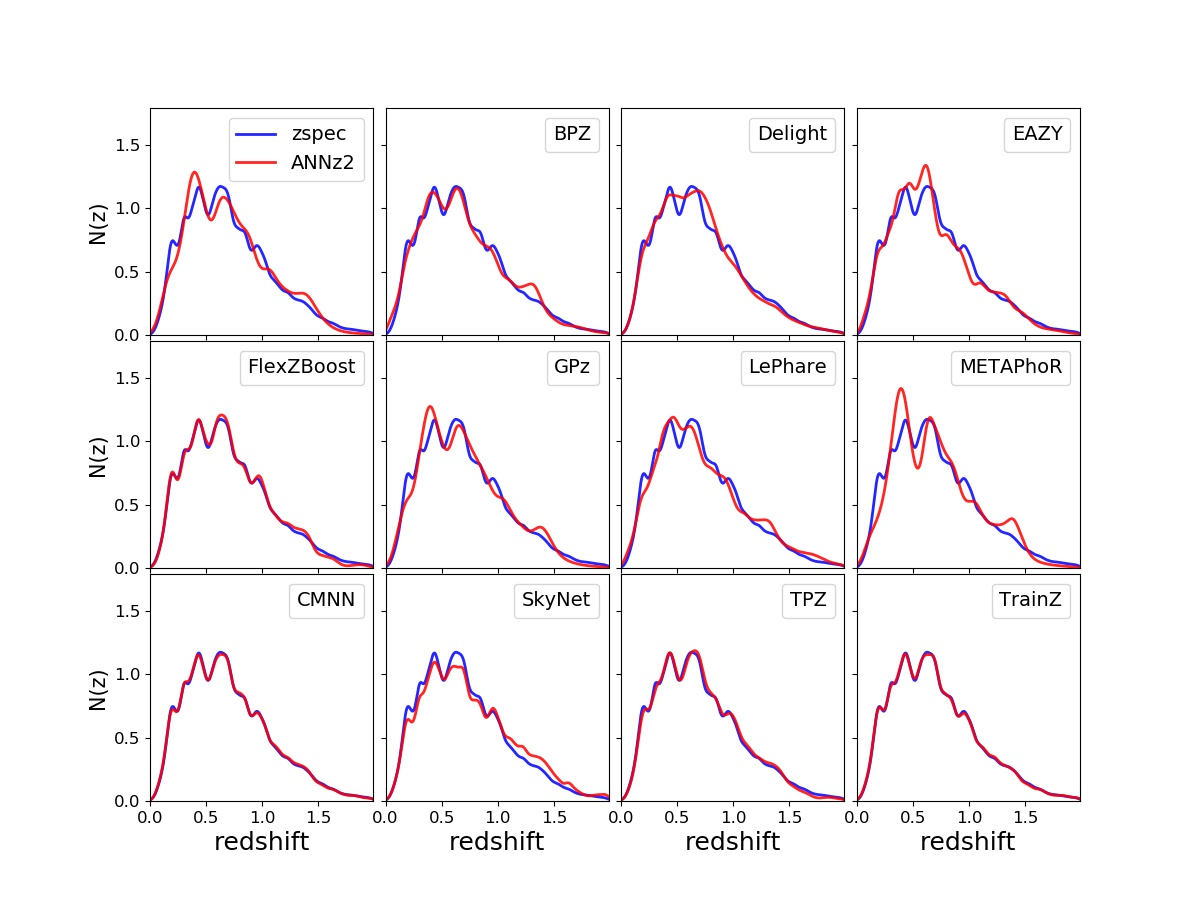
\includegraphics[width=0.74\textwidth]{fig/NZsumplot_12codes_scottsrule_biglabels.jpg}
\caption{The smoothed stacked estimator $\hat{N}(z)$ of the redshift distribution (red) produced by each code (panels) compared to the true redshift distribution $\tilde{N}(z)$ (blue).
Varying levels of agreement are seen among the codes, with the smallest deviations for \cmnn, \flexzboost, \tpz, and \trainz.}
\label{fig:nz}
\end{figure*}

Many of the codes, including all the model-fitting approaches and \annz, \gpz, \metaphor, and \skynet\ from the data-driven camp, overestimate the redshift density at $z \sim 1.4$.
This behavior is a consequence of the $4000$ \AA\ break passing through the gap between the $z$ and $y$ filters, which induces a \sout{genuine discontinuity}\boldblue{dramatic rise and fall} in the $z - y$ colour as a function of redshift\boldblue{.  With a dearth of strong spectral features blue-ward of the 4000 \AA\ break in most galaxy SEDs, the degeneracies on either side of the peak in $z - y$ colour tend to broaden the redshift PDFs near $z \sim 1.4$, which can lead to the ``bump'' seen in the stacked $\hat{N}(z)$ estimate.} \sout{that can sway the \pzpdf\ estimates in the absence of bluer spectral features.}

\annz, \gpz, and \metaphor\ feature exaggerated peaks and troughs relative to the training set, a potential sign of overtraining.
Further investigation on overtraining is needed, if present this is an obstacle that may be overcome with adjustment of the implementation.

As expected, \trainz\ perfectly recovers the true redshift distribution: as the training sample is selected from the same underlying distribution as the test set, the redshift distributions are identical, up to Poisson fluctuations due to the finite number of sample galaxies.
\cmnn\ is also in excellent agreement for similar reasons: with a representative training sample of galaxies spanning the colour-space, the sum of the colour-matched neighbour redshifts should return the true redshift distribution.
\flexzboost\ and \tpz\ also perform superb recovery of the true redshift distribution, with only a slight deviation at $z \sim 1.4$.
\sout{Our metrics, however, cannot discern whether these four approaches, as well as \delight, are spared the $z \sim 1.4$ degeneracy in $\hat{N}(z)$ because they have more effectively used information in the data or if the impact is simply washed out by the stacked estimator's effective average over the test set galaxy sample.
See Appendix~\ref{sec:pointmetrics} for further discussion of the $z \sim 1.4$ issue.}

Figure~\ref{fig:nz_stats} shows the quantitative Kolmogorov-Smirnoff (KS), Cramer-Von Mises (CvM), and Anderson Darling (AD) test statistics for each of the codes for the $\hat{N}(z)$ based measures.
The horizontal lines show the the result of a bootstrap resampling of the training set using \sout{30}\boldblue{44},000 samples for \trainz, representing a conservative \sout{idealized limit on expected performance for a} \boldblue{error estimate assuming our} modest-sized representative training set of galaxies, as mentioned in Section~\ref{sec:pitqq}.
The AD bootstrap statistic is elevated due to its sensitivity to the tails of distributions.
The stacked estimators of the redshift distribution for \cmnn\ and \trainz\ best estimate $\tilde{N}(z)$ under these metrics, whereas \eazy, \lephare, \metaphor, and \skynet\ underperform; \bpz, \gpz, and \tpz\ are within a factor of two of the conservative limit for all statistics.
It is unsurprising that \cmnn\ scores well, as with a nearly complete and representative training set choosing neighbouring points in colour/magnitude space to construct an estimator should lead to excellent agreement in the final $\hat{N}(z)$.

\begin{figure*}
\centering
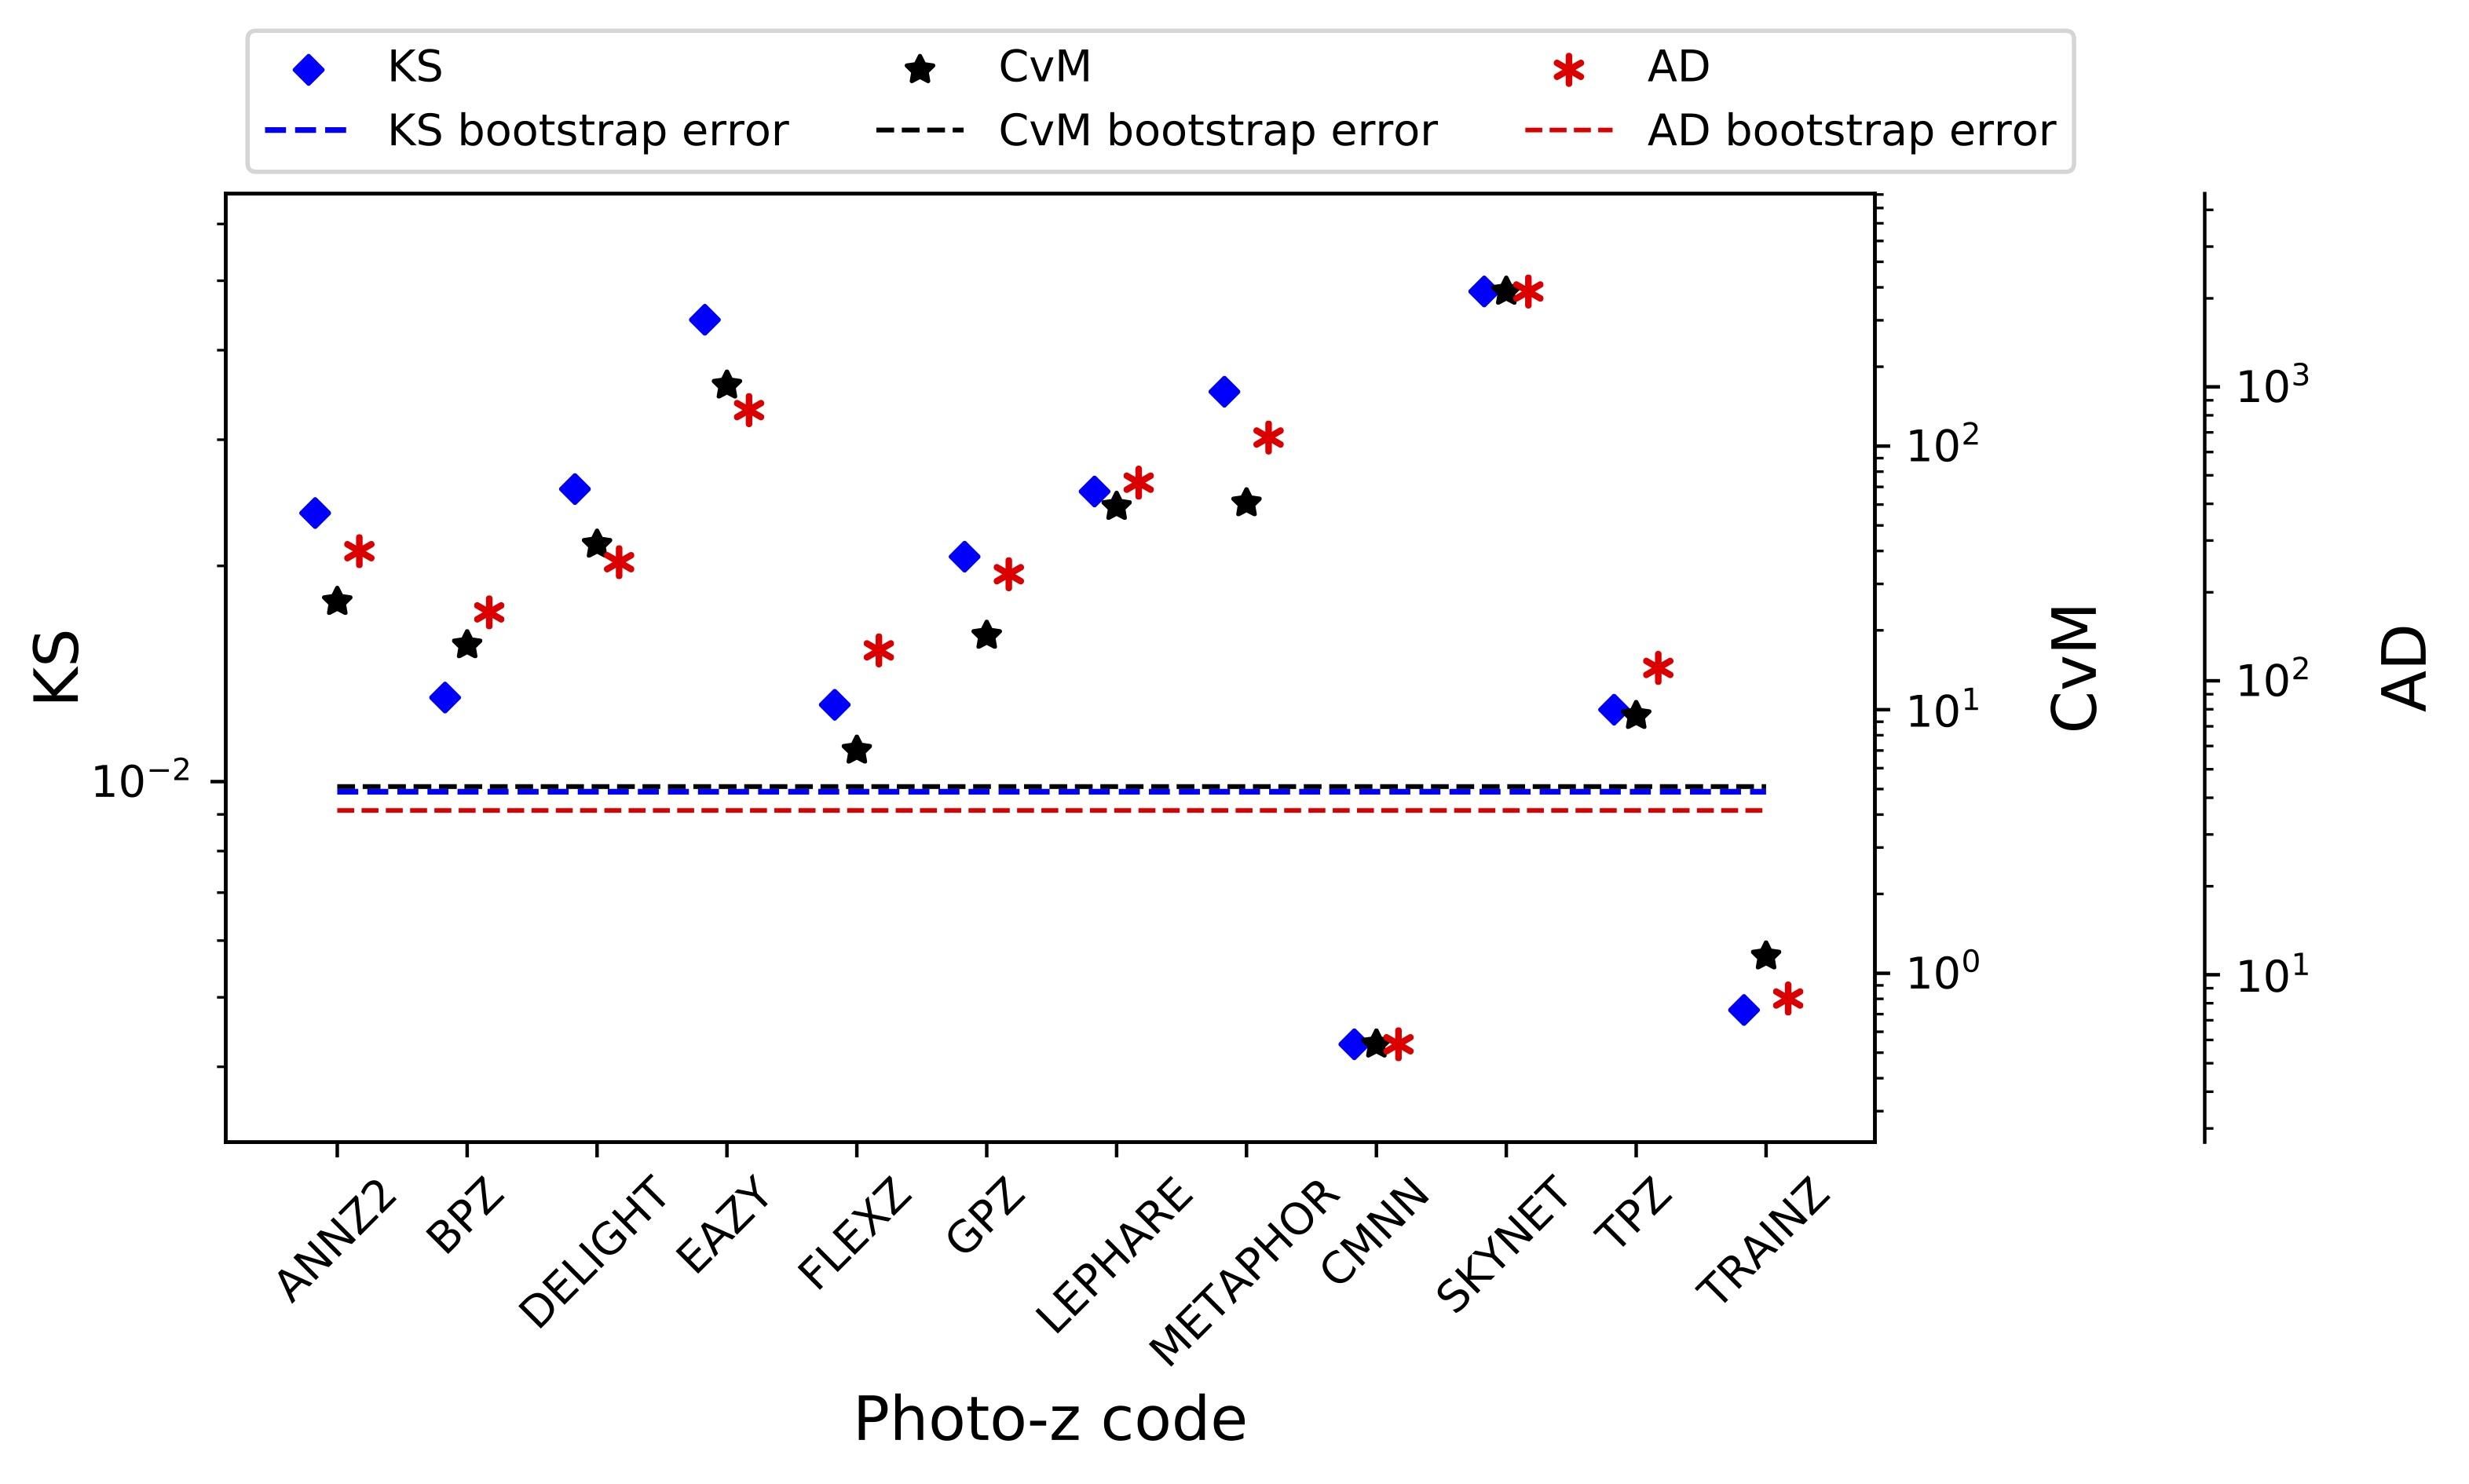
\includegraphics[width=0.74\textwidth]{fig/KSvsCvMvsAD_NZ_withnull_44k.jpg}
\caption{A visualization of the Kolmogorov-Smirnoff (KS, blue diamond), Cramer-von Mises (CvM, black star), and Anderson-Darling (AD, red asterisk) statistics for the $\hat{N}(z)$ distributions.
Horizontal lines indicate the statistic values (including uncertainty) achieved using \trainz\ via bootstrap resampling a training set containing \sout{30}\boldblue{44},000 redshifts.
We make the reassuring observation that these related statistics do not disagree significantly with one another.
\cmnn\ outperforms the control case, \trainz, and several codes are within a factor of two of this conservative idealized limit.
\skynet\ scores poorly due to an overall bias in its redshift predictions.}
\label{fig:nz_stats}
\end{figure*}

It is, however, surprising that \tpz\ does well on $\hat{N}(z)$ given its poor performance on the ensemble \pzpdf s, especially knowing that \tpz\ was optimized for \pzpdf\ ensemble metrics rather than the stacked estimator of the redshift distribution.
A possible explanation is the choice of smoothing parameter chosen during validation, which affects \pzpdf\ widths as well as overall redshift bias and could be modified to improve performance under the \pzpdf\ metrics.

\begin{figure*}
\centering
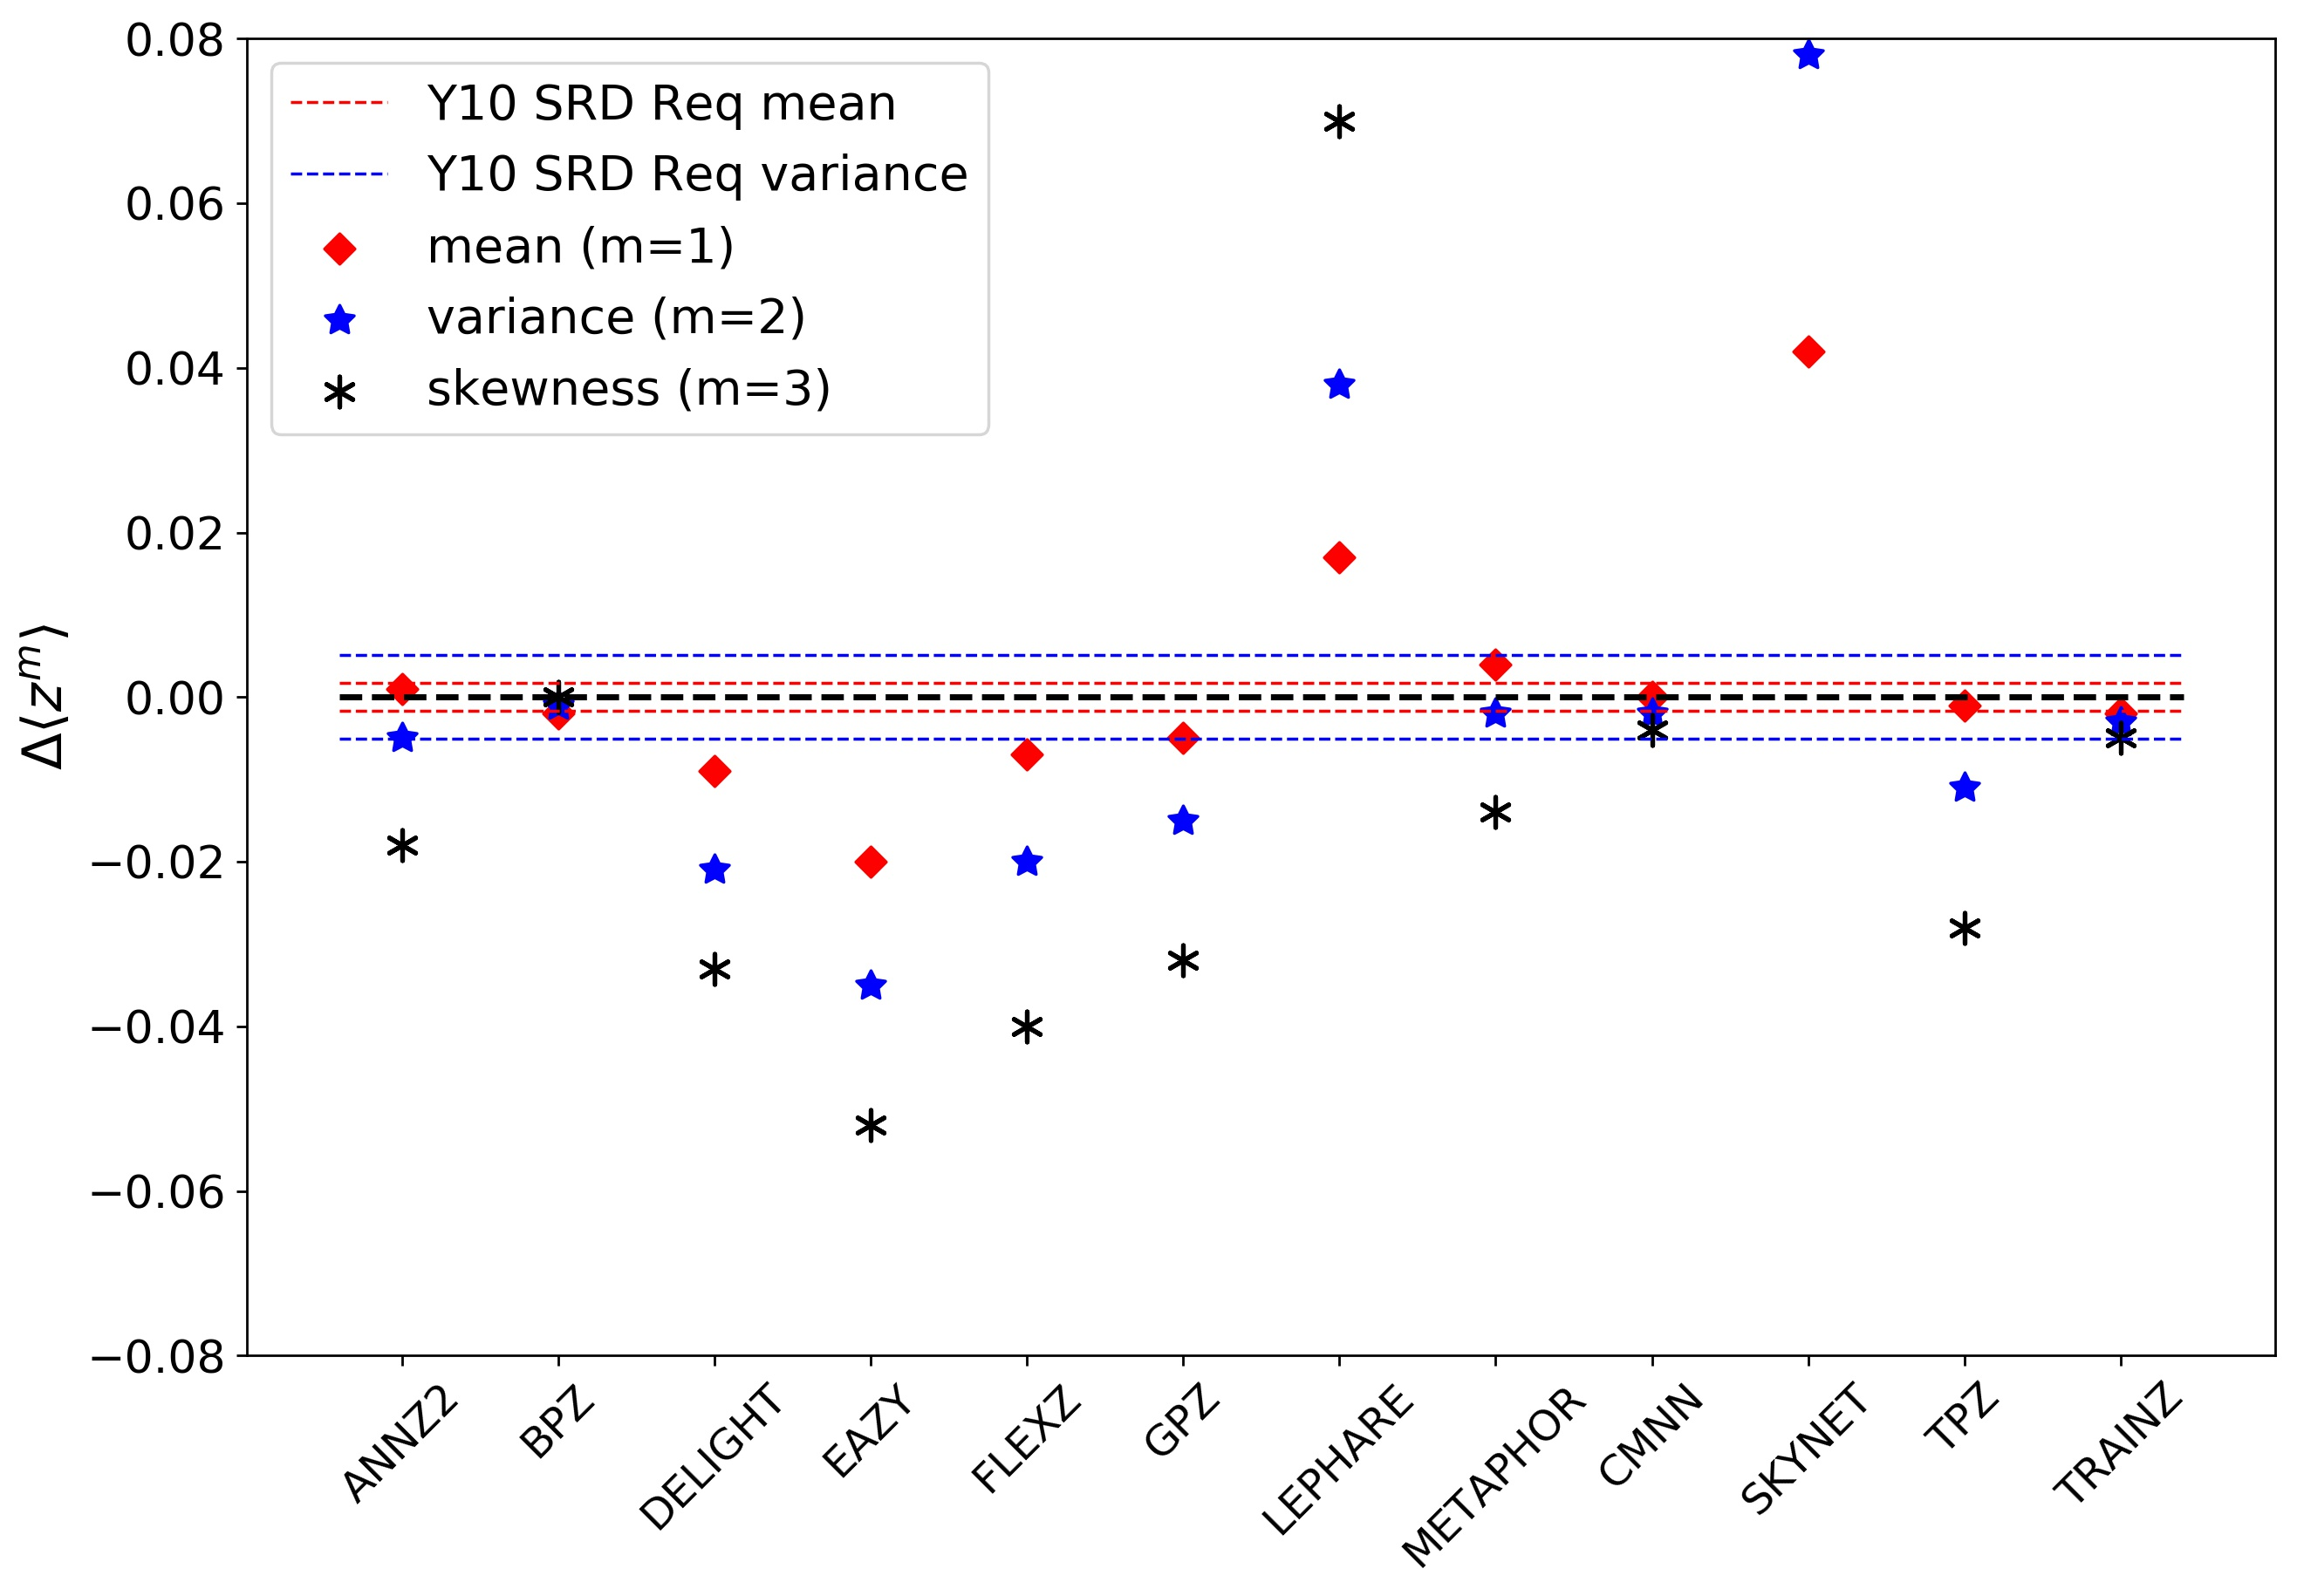
\includegraphics[width=0.75\textwidth]{fig/momentsplot_10yr.jpg}
\caption{Residuals of the first three moments of the stacked $\hat{N}(z)$ distribution.  Red and blue horizontal lines indicate the Year 10 DESC SRD requirements on accuracy of the mean and variance respectively.  Only a small number of codes are able to meet these specifications even with perfect training data.   }
\label{fig:moments}
\end{figure*}


We calculated the first three moments of the stacked $\hat{N}(z)$ distribution of all galaxies and compared it to the moments of the true redshift distribution.  Figure~\ref{fig:moments} shows the residuals of the moments for all codes.  Accuracy of the moments varies widely between codes, raising concerns about the propagation to cosmological analyses.  The DESC SRD \citep{Mandelbaum:2018} lists stringent requirements on how well the mean and variance of tomographic redshift bins must be known for each of the main DESC science cases.  We indicate the Year 10 (Y10) requirements assuming our true mean redshift of $z=0.701$ as dashed lines.  In this study with representative training data, \annz, \cmnn, \tpz, and our pathological \trainz\ estimator meet the Y10 requirement on the mean redshift.  Only \annz, \cmnn, and \trainz\ meet both requirements.  One should be concerned that many codes fail to meet this ambitious limit under perfect prior information because all codes are anticipated to do no better under realistically imperfect prior information, and indicates that additional calibration to remove these systematic offsets \citep[e.~g.~][]{Newman:2008} will likely be necessary in order to meet these stringent goals.


\skynet\ exhibits redshift bias in Figure~\ref{fig:nz} and is a clear outlier in the first moment of $\hat{N}(z)$ in Figure~\ref{fig:moments}.
The \skynet\ algorithm employs a random subsampling of the training set without testing that the subset is representative of the full population, and the implementation used here does not upweight rarer low- and high-redshift galaxies, as in \citet{Bonnett:15}, suggesting a possible cause that may be addressed in future work.

\section{\Pz\ point estimation and metrics}
\label{sec:pointmetrics}

While this work assumes that science applications value the information of the full \pzpdf, we present conventional metrics of \pz\ point estimates as a quick and dirty visual diagnostic tool and to facilitate direct comparisons to historical studies.

\subsection{Reduction of \pzpdf s to point estimates}
\label{sec:pointest}

Though we acknowledge that many of the codes can also return a native \pz\ point estimate, we put all codes on equal footing by considering two generic \pz\ point estimators, the mode $z_{PEAK}$ and main-peak-mean $z_{WEIGHT}$ \citep{Dahlen:13}, a weighted mean within the bounds of the main peak, as identified by the roots of $p(z) - 0.05 \times z_{PEAK}$.
Though $z_{WEIGHT}$ neglects information in a secondary peak of e.~g.~ a bimodal distribution, it avoids the pitfall of reducing the \pzpdf\ to a redshift between peaks where there is low probability.

\subsection{Metrics of \pz\ point estimates}
\label{sec:point_metrics}

We calculate the commonly used point estimate metrics of the overall intrinsic scatter, bias, and catastrophic outlier rate, defined in terms of the standard error $e_{z} \equiv (z_{PEAK} - z_{\mathrm{true}}) / (1 + z_{\mathrm{true}})$.
Because the standard deviation of the \pz\ residuals is sensitive to outliers, we define the scatter in terms of the Interquartile Range (IQR), the difference between the 75th and 25th percentiles of the distribution of $e_{z}$, imposing the scaling $\sigma_{\mathrm{IQR}} = \mathrm{IQR} / 1.349$ to ensure that the area within $\sigma_{\mathrm{IQR}}$ is the same as that within one standard deviation from a standard Normal distribution.
We also resist the effect of catastrophic outliers by defining the bias $b_{z}$ as the median rather than mean value of $e_{z}$.
The catastrophic outlier rate $f_{\mathrm{out}}$ is defined as the fraction of galaxies with $e_{z}$ greater than $\max(3 \sigma_{\mathrm{IQR}}, 0.06)$.

For reference, Section 3.8 of the \lsst\ Science Book \citep{Abell:09} uses the standard definitions of these parameters in requiring
\begin{itemize}
\item RMS scatter $\sigma < 0.02 (1 + z_{\mathrm{true}})$
\item bias $b_{z} < 0.003$ 
\item catastrophic outlier rate $f_{\mathrm{out}} < 10$ per cent 
\end{itemize}

\subsection{Comparison of \pz\ point estimate metrics}
\label{sec:pointmetrics_results}

Figure~\ref{fig:pz_pointestimates} shows \sout{both} point estimates \sout{both} $z_{PEAK}$ and $z_{WEIGHT}$ \boldblue{versus true redshift for all codes}.
Point density is shown with mixed contours to emphasize that most of the galaxies do fall close to the $z_{phot} = z_{spec}$ line, while points trace the details of the catastrophic outlier populations.

\begin{figure*}
\centering
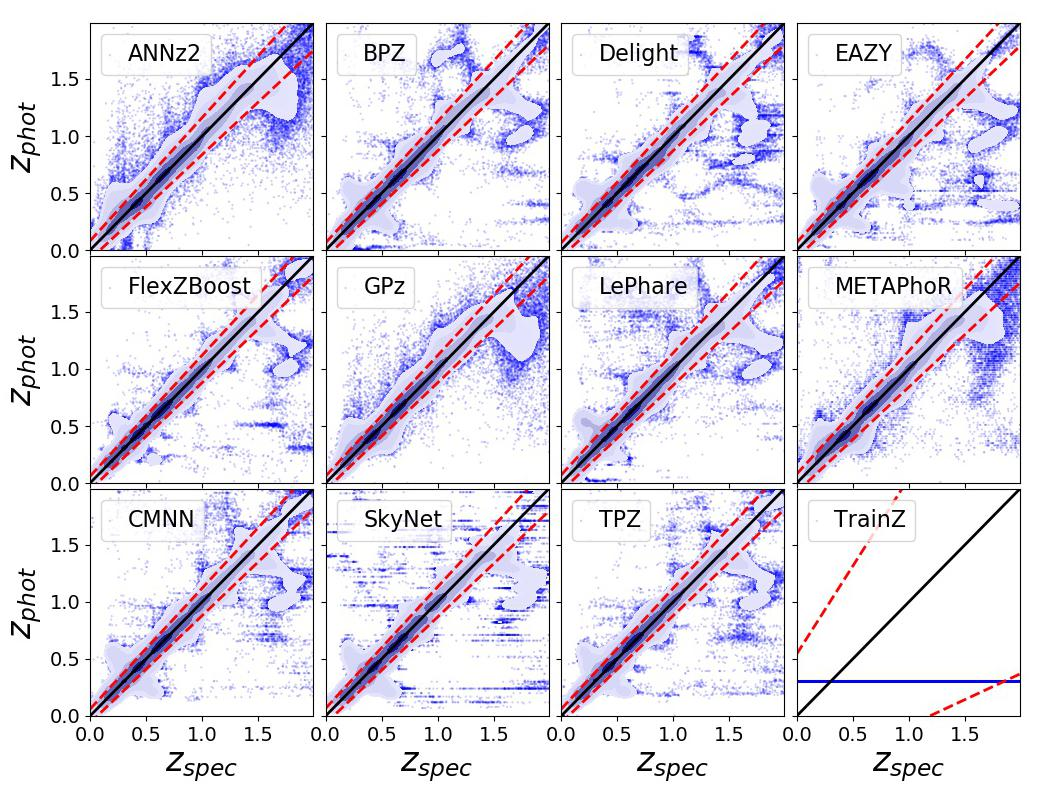
\includegraphics[width=0.49\textwidth]{fig/ZPEAK_szpz_threecolumn_12codes_biglabels_crop.jpg}
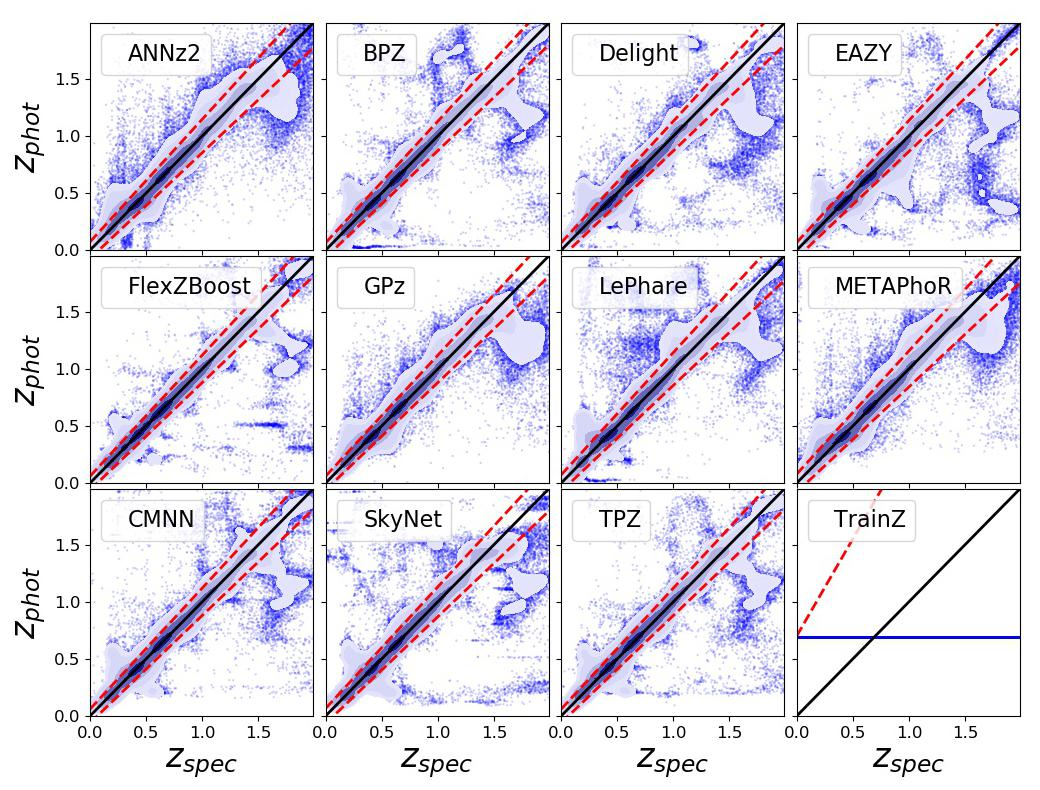
\includegraphics[width=0.49\textwidth]{fig/ZWEIGHT_szpz_threecolumn_12codes_biglabels_crop.jpg}
\caption{The density of \pz\ point estimates (contours) reduced from the \pzpdf s with outliers (blue) beyond the outlier cutoff (red dashed lines), via the mode ($z_{PEAK}$, left panel) and main-peak-mean ($z_{WEIGHT}$, right panel).
The \trainz\ estimator (lower right sub-panels) has a shared $z_{PEAK}$ and $z_{WEIGHT}$ for the entire test set galaxy sample.}
\label{fig:pz_pointestimates}
\end{figure*}

The finite grid spacing of the \pzpdf s induces some discretization in $z_{PEAK}$.
The features perpendicular to the $z_{phot} = z_{spec}$ line are due to the $4000$ \AA\ break passing through the gaps between adjacent filters\boldblue{,  most notably at $z \sim 0.4$ between the g and r filters, and at $z \sim 1.4$ between the z and y filters.  All codes show some level of concentrated catastrophic outliers, often due to degenerate redshift solutions for a single area of color space.  In the presence of genuine ambiguities in the colour space to redshift mapping, the compression of information down to a single number that is the point estimate redshift fails to adequately capture the more complex nature of the multimodal redshift matching: using the mode selects the highest peak while ignoring posterior probability in lower valued redshift peaks, while measuring the mean of a multimodal PDF often results in a value lying at a redshift between the peaks, removed from either/any of the most likely redshift solutions.  Thus,} \sout{E}even the strongest codes feature populations far from the $z_{phot} = z_{spec}$ line representing a \boldblue{genuine} degeneracy in the space of colours and redshifts.

\begin{table*}
\begin{center}
\caption{\Pz\ point estimate statistics}\label{tab:pointestimates}
\begin{tabular}{lcccccc}
\hline
\hline
                 &            & $Z_{PEAK}$  &          &  & $Z_{WEIGHT}$          &\\
\hline
\Pzpdf\ Code       & $\frac{\sigma_{IQR}}{(1+z)}$ & median  & \multicolumn{1}{|p{0.75cm}|}{\centering outlier \\fraction} & $\frac{\sigma_{IQR}}{(1+z)}$ & median & \multicolumn{1}{|p{0.75cm}|}{\centering outlier \\fraction}\\
\hline
\annz     & 0.0270  &  0.00063  & 0.044      & 0.0244  &  0.000307  & 0.047  \\
\bpz       & 0.0215  & -0.00175  & 0.035      & 0.0215  & -0.002005  & 0.032 \\
\delight   & 0.0212  & -0.00185  & 0.038      & 0.0216  & -0.002158  & 0.038 \\
\eazy      & 0.0225  & -0.00218  & 0.034      & 0.0226  & -0.003765  & 0.029 \\
\flexzboost& 0.0154  & -0.00027  & 0.020      & 0.0148  & -0.000211  & 0.017 \\
\gpz       & 0.0197  & -0.00000  & 0.052      & 0.0195  &  0.000113  & 0.051 \\
\lephare   & 0.0236  & -0.00161  & 0.058      & 0.0239  & -0.002007  & 0.056 \\
\metaphor  & 0.0264  &  0.00000  & 0.037      & 0.0262  &  0.001333  & 0.048 \\
\cmnn        & 0.0184  & -0.00132  & 0.035      & 0.0170  & -0.001049  & 0.034 \\
\skynet    & 0.0219  & -0.00167  & 0.036      & 0.0218  &  0.000174  & 0.037 \\
\tpz       & 0.0161  &  0.00309  & 0.033      & 0.0166  &  0.003048  & 0.031 \\
\hline
\trainz	   & 0.1808  &  -0.2086  & 0.000	  & 0.2335  & 0.022135  & 0.000\\
\end{tabular}
\end{center}
\end{table*}

The intrinsic scatter, bias, and catastrophic outlier rate are given in Table~\ref{tab:pointestimates}.
Perhaps unsurprisingly, performance under these metrics largely tracks that of the metrics of Section~\ref{sec:metrics} of the \pzpdf s from which the point estimates were derived.
All twelve codes perform at or near the goals of the \lsst\ Science Requirements Document\footnote{available at: \url{http://ls.st/srd}} and \citet{Graham:17}, which is encouraging if not unexpected for $i < 25.3$.



\bibliography{main,lsstdesc}

\end{document}

% ======================================================================
